\chapter*{\textbf{Capítulo III: Metodología}}
\addcontentsline{toc}{chapter}{\textbf{III. Metodología}}
\chead{Metodología}
\setcounter{chapter}{3}

En este capítulo se expone la metodología seguida para la obtención de los resultados de este trabajo, adem\'as de los conocimientos teóricos básicos y las herramientas numéricas para el análisis de los datos obtenidos.


\section*{III.1 Datos observacionales, estudios preparatorios para TAOS-II}
\addcontentsline{toc}{section}{III.1 Datos observacionales, estudios preparatorios para TAOS-II}

Este trabajo está pensado para llevarse acabo con datos del proyecto TAOS-II, cuando entre en completo funcionamiento. Como parte de este trabajo de tesis, se realizaron observaciones de tránsitos de exoplanetas a una cadencia de 20 fps, es decir, bajo las mismas condiciones que se tendrán en TAOS-II \cite{lehner2012transneptunian}. Todo esto con el fin, de que cuando el proyecto comience, se tengan las herramientas y metodología para analizar los datos.

Hay que destacar que TAOS-II tendrá curvas de luz de 2 horas de duraci\'on por campo de observación, esto para observar con la menor masa de aire posible. Debido a esto será muy difícil observar un tránsito completo, se espera observar la entrada o la salida del exoplaneta frente al disco estelar. 

A una cadencia de 20 fps, esto se traduce en curvas con $N=144,000$ muestras. Además, por campo de observación se espera observar alrededor de 10,000 estrellas simultáneamente. Por este motivo, los análisis y la metodología presentadas en este trabajo, se enfocan en detectar las firmas de tránsitos de exoplanetas de la manera más eficiente posible.

\subsection*{III.1.1 Telescopio e instrumentos en la temporada de observación}
\addcontentsline{toc}{subsection}{III.1.1 Telescopio e instrumentos en la temporada de observación}

La mayoría de las observaciones se realizaron en el telescopio de $84~cm$ en el OAN-SPM (Figura 3.1). Utilizando la rueda de filtros MEXMAN, este instrumento permite intercambiar el filtro que se antepone al detector. En total se cuenta con dos ruedas de filtros con 8 posiciones, lo cual resulta en 14 filtros en total (dos posiciones están normalmente vacías). 

Como detector se utilizaron dos cámaras en distintas temporadas. La primera de ellas fue del 1-6 de agosto del 2016, usando una cámara rápida iXon Ultra 888 de la marca ANDOR, capaz de tomar imágenes de muy corta exposición, con cadencias de hasta 300 imágenes por segundo (fps del inglés \textit{frames per second}). Esta cámara es la única disponible en el OAN-SPM que puede trabajar a 20 fps. A su vez, las imágenes se tomaron en un \textit{binning}\footnote{Binning es una manera de medir el CCD, uniendo la constibución de varios pixeles adyacentes.} de 3x3, con esto, se logró igualar la escala de placa del telescopio de 84 cm, con los telescopios de TAOS-2 en donde el campo de visión fue de $~3.5$ minutos de arco.

\begin{figure}[h!]
\centering
  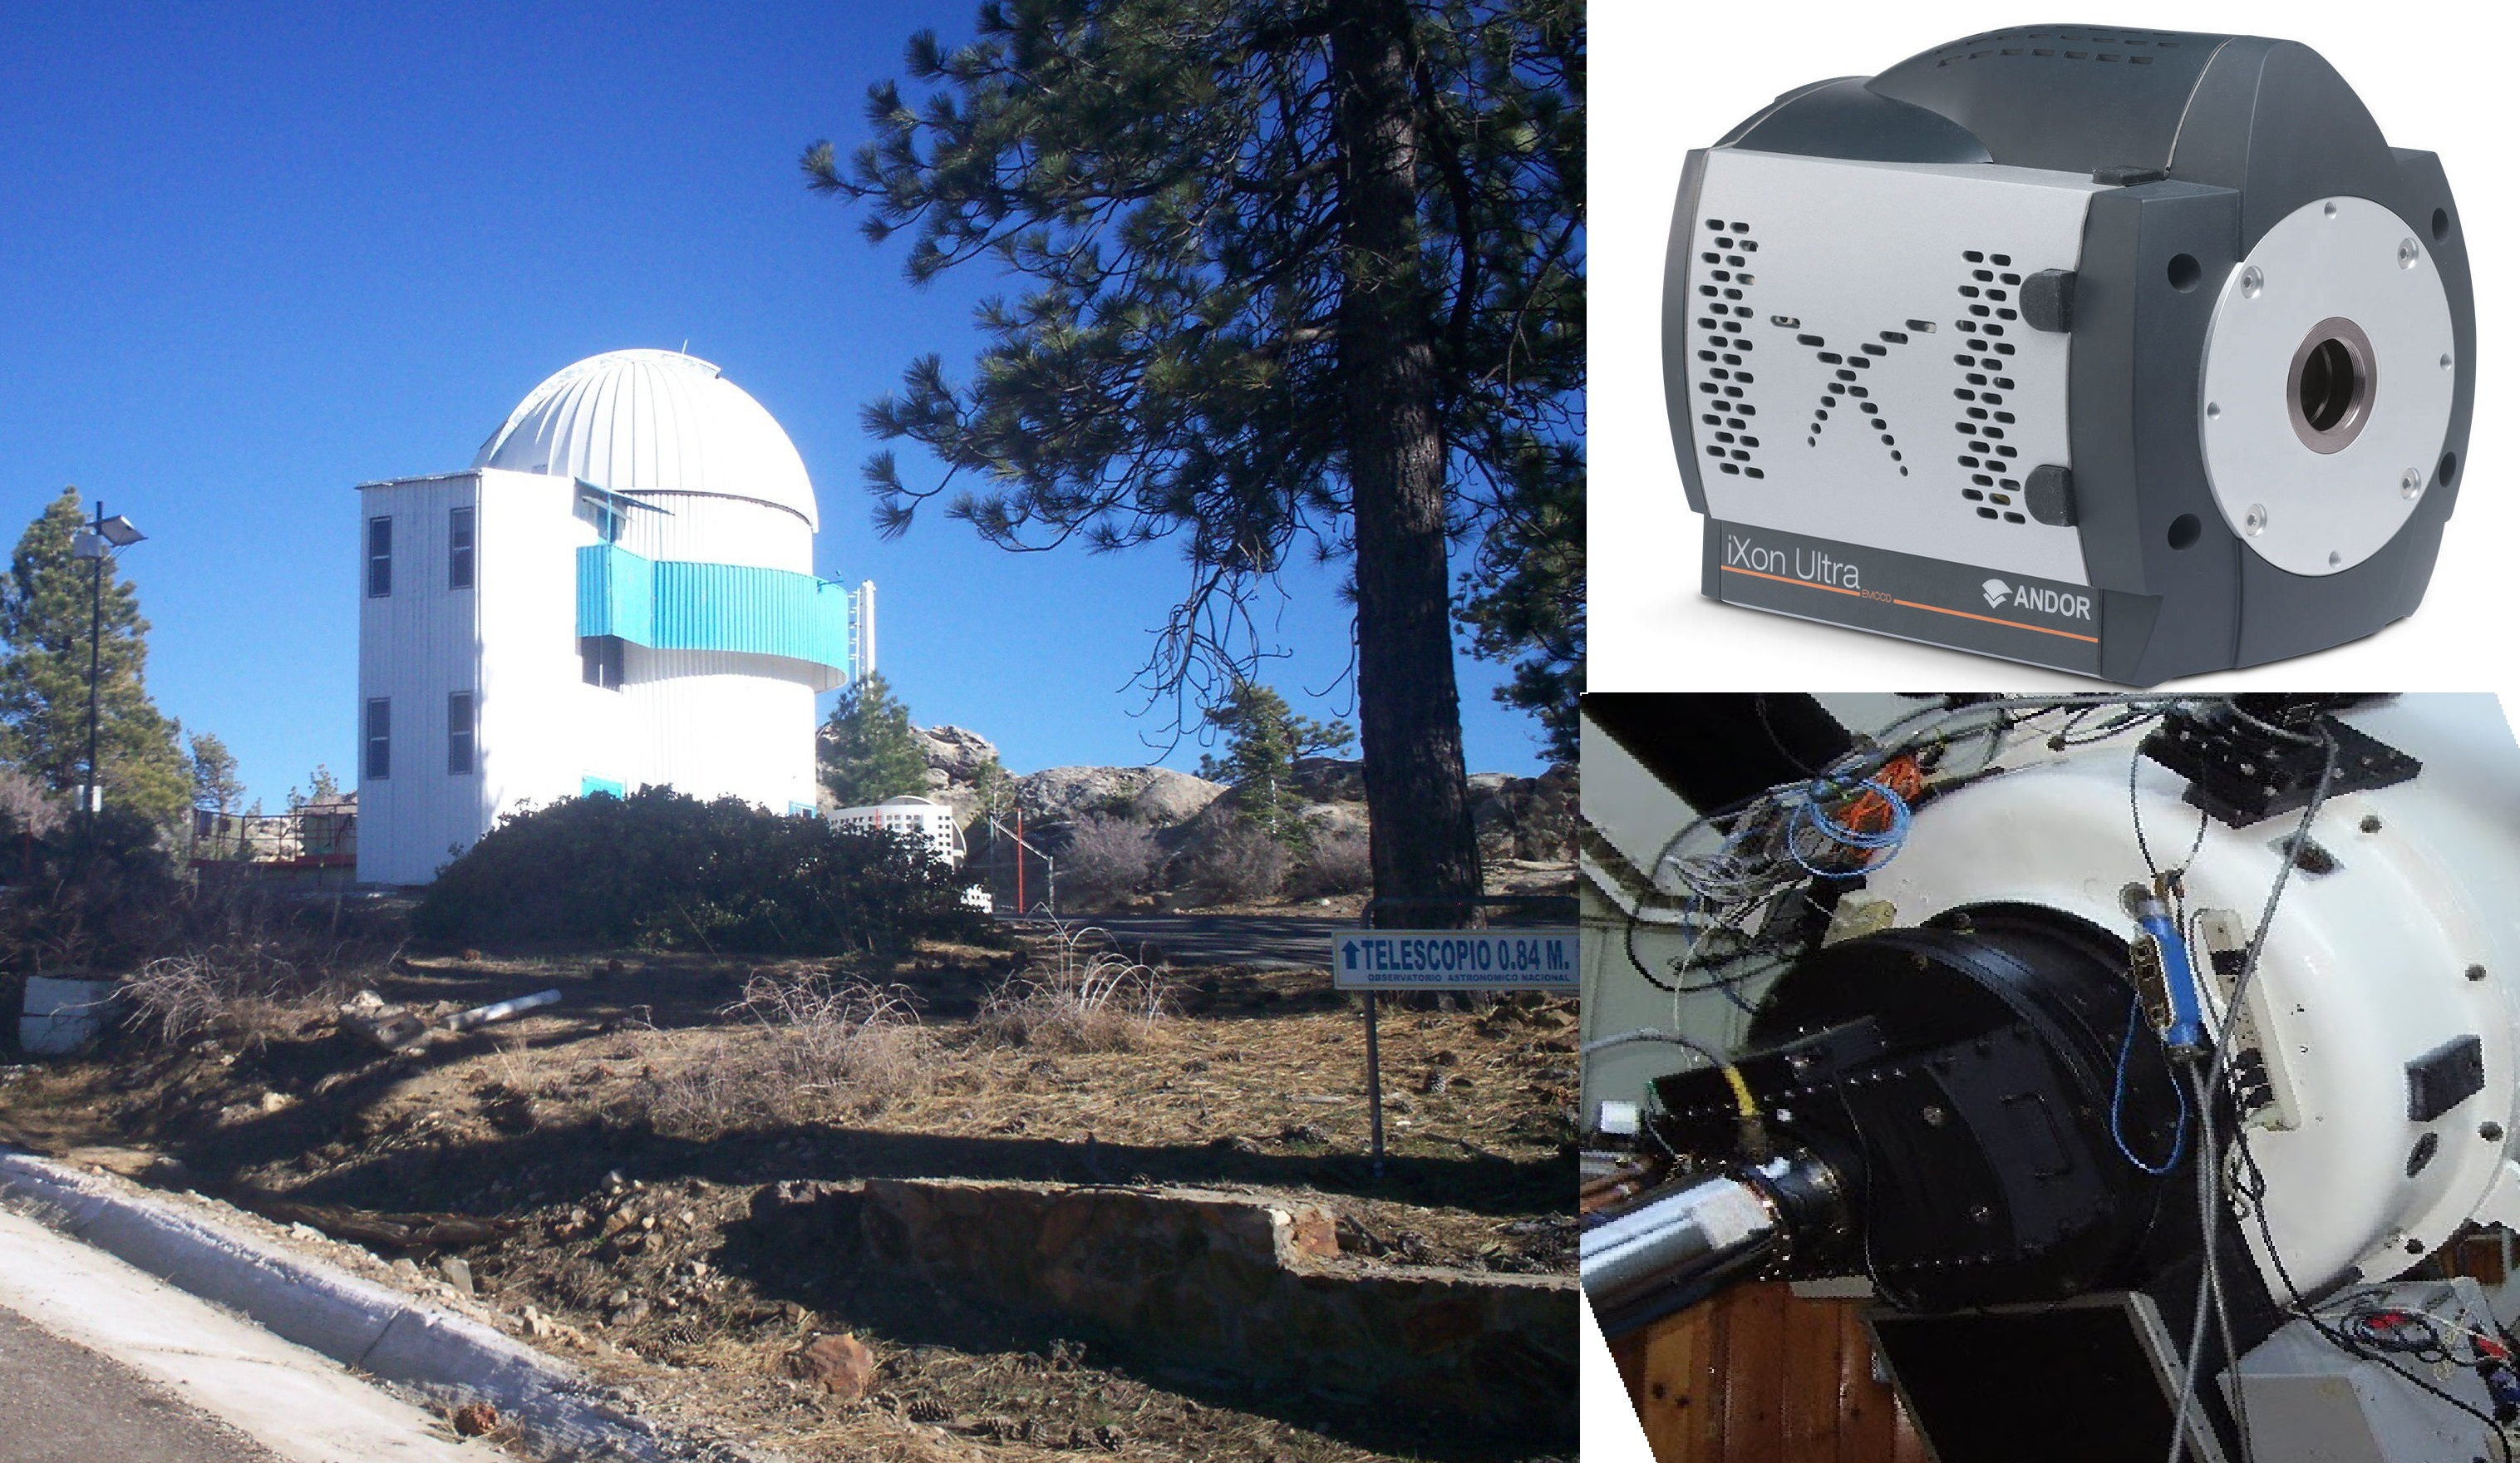
\includegraphics[max size={0.7\textwidth}{0.7\textheight}]{./figures/84cm.jpg}
 \caption{Fig. 3.1. Telescopio de 84 cm, en el OAN-SPM, cámara rápida iXon y rueda de filtros MEXMAN.}
  \label{fig:3.1}
\end{figure}

La segunda temporada de observación ocurrió del 26-05 de junio del 2017, igualmente en el telescopio de 84 cm. El detector fue una cámara \textit{frame transfer} de la marca \textit{Spectral Instruments}. El campo de la cámara fue disminuido para alcanzar la cadencia necesaria (20 fps), al igual el \textit{binning} de las imágenes variaba dependiendo de la magnitud de la estrella.

\textcolor{red}{no vamos a presentar nada de los telescopios de TAOS II???}

\subsection*{III.1.2 Descripción de objetos observados}
\addcontentsline{toc}{subsection}{III.1.2 Descripción de objetos observados}

A continuación en la Tabla 3.1 se muestra un resumen de los parámetros de los objetivos observados en las múltiples temporadas, algunos objetivos fueron observados en varias ocasiones y bajo distintas condiciones dependiendo del detector utilizado.



\begin{table}
\hspace{-1.7cm}
\begin{footnotesize}
\begin{tabular}{ccccccccc}
\hline 
 & \multicolumn{4}{c}{Parámetros del} & \multicolumn{3}{c}{Parámetros de la} &  \\
 & \multicolumn{4}{c}{planeta} & \multicolumn{3}{c}{estrella} & \\
\hline 
Nombre & $M_{p} (M_{J}) $ & $R_{p} (R_{J}) $ &  P (días) & $\Delta F (\%)$ & $M_{*} (M_{\odot})$ & $M_{v}$ & $T_{s}$ & Referencia \\ 
\hline 
HAT-P-14b & $2.2\pm 0.04 $ & $1.2\pm 0.04 $ & 4.62 & 0.55 & $1.38\pm 0.045$ & 9.9 & F & \cite{torres2010hat} \\ 
HAT-P-31b & $2.1^{+0.105}_{-0.07} $ & $1.07^{+0.24}_{-0.16} $ & 5 & 1.08 & $1.21\pm 0.063$ & 11.6 & - & \cite{kipping2011hat} \\
HAT-P-32b & $0.86^{+0.105}_{-0.07} $ & $1.79\pm 0.025 $ & 2.15 & 2.44 & $1.12\pm 0.07$ & 11.29 & F/G & \cite{hartman2011hat} \\  
HAT-P-37b & $1.1\pm 0.103 $ & $1.17\pm 0.07 $ & 2.79 & 2.04 & $0.92\pm 0.043$ & 13.2 & - & \cite{bakos2012hat} \\
WASP-48b & $0.98\pm 0.09 $ & $1.6\pm 0.08 $ & 2.14 & 1.08 & $1.19\pm 0.05$ & 11.06 & - & \cite{enoch2011wasp} \\
WASP-74b & $0.82\pm 0.014 $ & $1.4\pm 0.018 $ & 2.13 & 1.04 & $1.48\pm 0.12$ & 9.7 & F9 & \cite{hellier2015three} \\
WASP-3b & $2.6\pm 0.13 $ & $1.45\pm 0.084 $ & 1.84 & 1.23 & $1.24\pm 0.11$ & 10.6 & F7V & \cite{pollacco2008wasp} \\
Kepler 17b & $2.45\pm 0.014 $ & $1.31\pm 0.018 $ & 1.48 & 2.13 & $1.16\pm 0.06$ & 14 & G2V & \cite{desert2011hot} \\
\hline 
\end{tabular} 
\end{footnotesize}
\caption{Tabla 3.1. Resumen de propiedades físicas de los objetos observados en distintas temporadas en el OAN-SPM. $M_{p}$ es la masa del planeta en unidades de masas de Júpiter, $R_{p}$ es el radio del planeta en radios de Júpiter, P es el periodo orbital en días, $\Delta F$ es el cambio en el flujo de la estrella debido al transito en porcentaje, $M_{*}$ es la masa de la estrella anfitriona en unidades de masas solares, $M_{v}$ y $T_{s}$ son la magnitud y el tipo espectral de la estrella respectivamente.}
\label{tab:tab_objetivos}
\end{table}

\subsection*{III.1.3 Descripción de datos, influencia del seeing y ruido sistemático}
\addcontentsline{toc}{subsection}{III.1.3 Descripción de datos, influencia del seeing y ruido sistemático}


Debido al corto tiempo de exposición, el número de cuentas por estrella es pequeño, por lo cual, el ruido electr\'onico se vuelve un factor importante. Por otro lado, las perturbaciones atmosf\'ericas afectan el \textit{seeing} que es una medida de la estabilidad de la atm\'osfera. Esto afecta a las im\'agenes de alta cadencia de dos maneras: 1) cambiando de posici\'on la estrella en el detector o deform\'andola, lo cual se convierte en una fuerte contribici\'on al ruido cuando se lleva a cabo la fotomtr\'ia de apertura. El \textit{seeing} durante las temporadas fue bueno, aunque se presentan ligeras variaciones en la posición de la estrella de toma a toma, este es el motivo por el cual no vemos la estrella como una circunferencia perfecta. Este ruido se ve reflejado a la hora de obtener la curva de luz de las imágenes. La cantidad de ruido se puede cuantificar calculando la SNR (2.11), la cual está en función de la magnitud aparente de la estrella.

\begin{figure}[H]
  \centering
    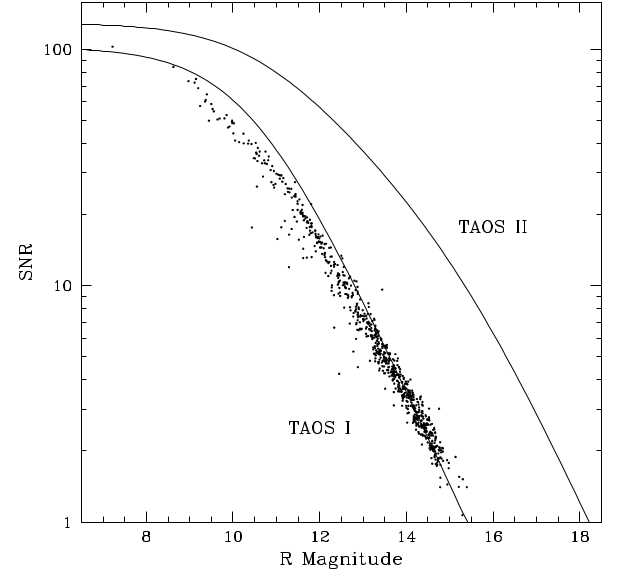
\includegraphics[max size={0.7\textwidth}{0.6\textheight}]{./figures/snr_vs_mag.png}
   \caption{Fig. 3.2. SNR en función de la magnitud en el filtro R. Los puntos representan la SNR calculada utilizando curvas de luz obtenidas en TAOS I. Las lineas solidas representan la predicción de SNR utilizando ruido con distribución de Poisson, ruido del cielo y ruido de lectura. Gr\'afica tomada de \cite{lehner2016status}.}
    \label{fig:3.2}
  \end{figure}


Utilizamos fotometría diferencial para reducir los sistemáticos, sin embargo no todos los campos observados contaban con buenas estrellas de comparación, por lo que en algunos casos se utilizó simplemente fotometría de apertura. Como se aprecia en las Figuras \ref{fig_2_6_foto_apertura} y \ref{fig_2_7_foto_diferencial}, las curvas de luz resultantes están dominadas por ruido. El propósito de este trabajo de tesis es idear metodologías para caracterizar el ruido y removerlo de las curvas de luz para poder detectar tránsitos de exoplanetas, es decir, detectar variaciones en el flujo de $(\sim 1-2 \%)$.

\section*{III.2 Análisis de ruido en curvas de luz de alta cadencia}
\addcontentsline{toc}{section}{III.2 Análisis de ruido en curvas de luz de alta cadencia}

A continuación se muestra la metodología para la caracterización del ruido, utilizando las curvas de luz resultantes de las temporadas de observación.

\subsection*{III.2.1 Distribución temporal del ruido}
\addcontentsline{toc}{subsection}{III.2.1 Distribución temporal del ruido}

El primer paso para la caracterización del ruido, fue saber que tipo de distribuciónes podemos encontrar en los datos. En esta subsección analizaremos el ejemplo de la curva de luz de WASP-74b (ver Tabla \ref{tab:tab_objetivos} para más detalle) calculada usando fotometría diferencial de las imágenes obtenidas el 27 de mayo del 2017. La metodología explicada a continuación se utiliz\'o para caracterizar el ruido en todas las curvas de luz.

\begin{equation}
  \displaystyle G(x)=Ae^{-\dfrac{(x-\mu)^{2}}{2\sigma^{2}}};
\end{equation}

Un ruido con una distribución gaussiana (3.1) es conocido como ruido blanco. Se puede apreciar un ejemplo en la Figura 3.3.

\begin{figure}[H]
  \centering
    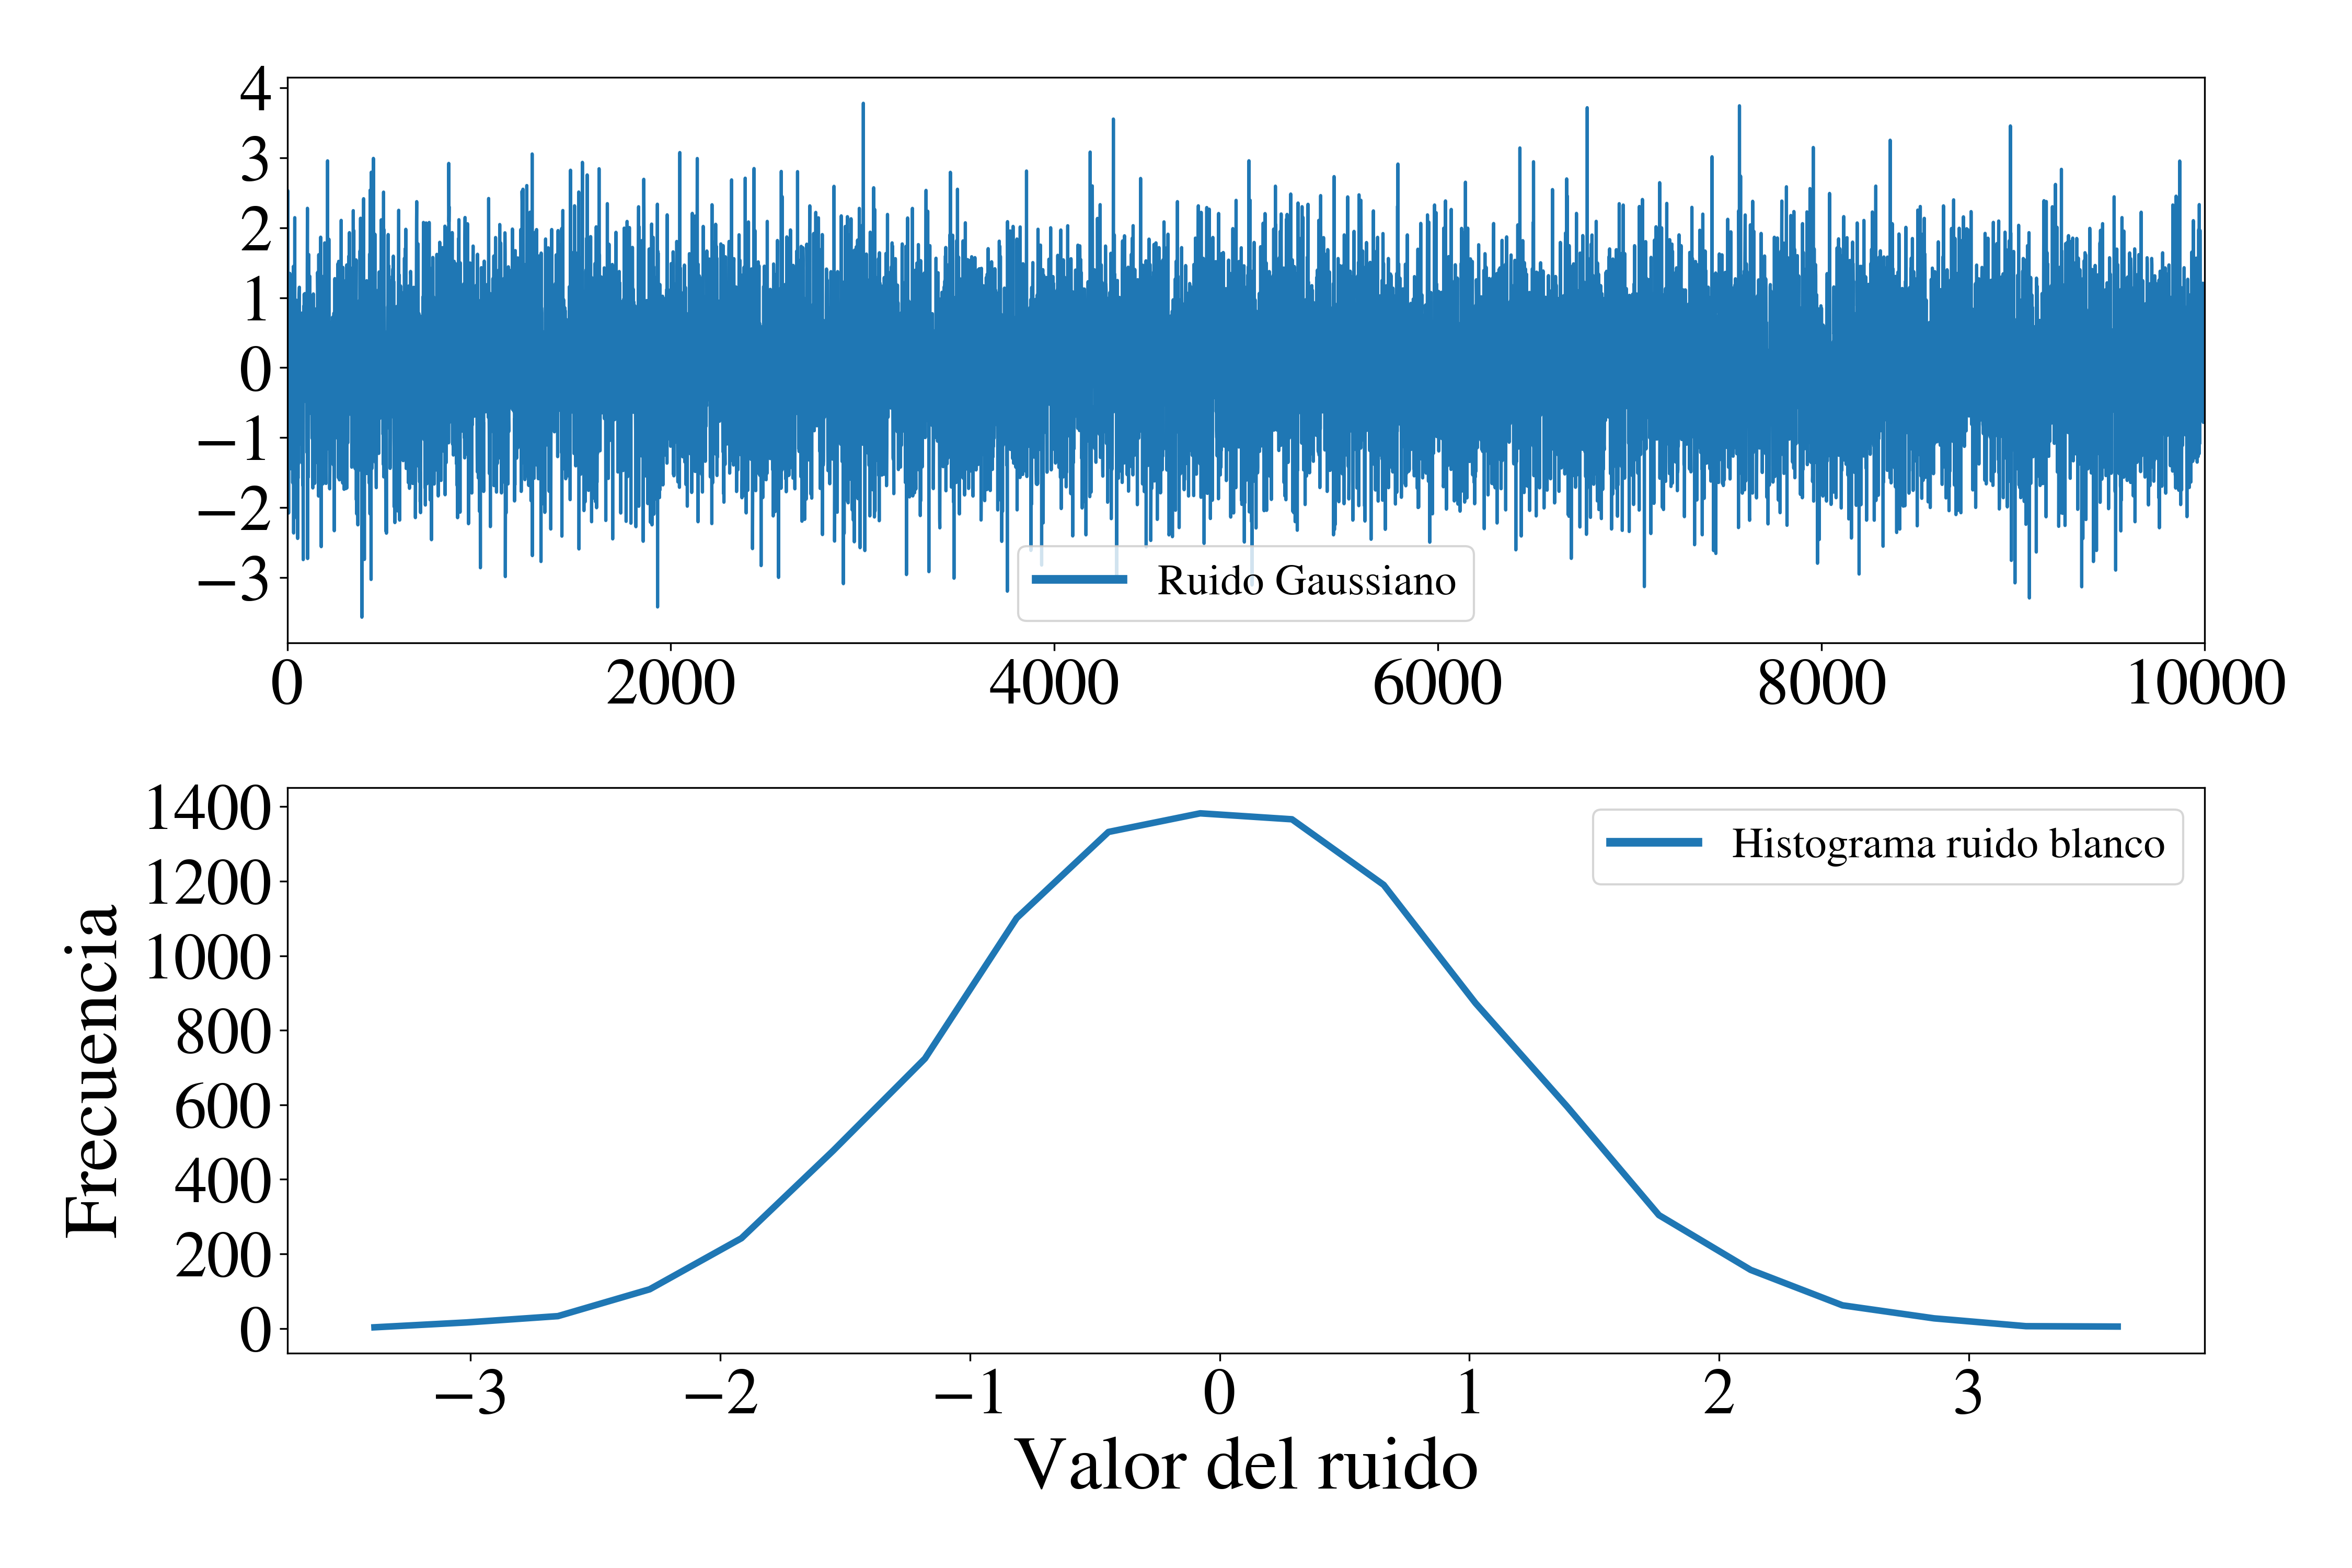
\includegraphics[max size={\textwidth}{0.7\textheight}]{./figures/ejemplo_ruido_gauss.png}
   \caption{Fig. 3.3. Arriba: Ejemplo de ruido blanco (gaussiano). Abajo: Histograma del ruido generado.}
    \label{fig:3.3_ruido_gauss}
\end{figure}

Esta es la manera mas común y simple de modelar el ruido, sin embargo, al analizar la curva de luz se encontraron 2 componentes gaussianas que conforman el ruido observado en la curva de luz de WASP-74b que se aprecia en la Figura 3.4.

\begin{figure}[H]
  \centering
    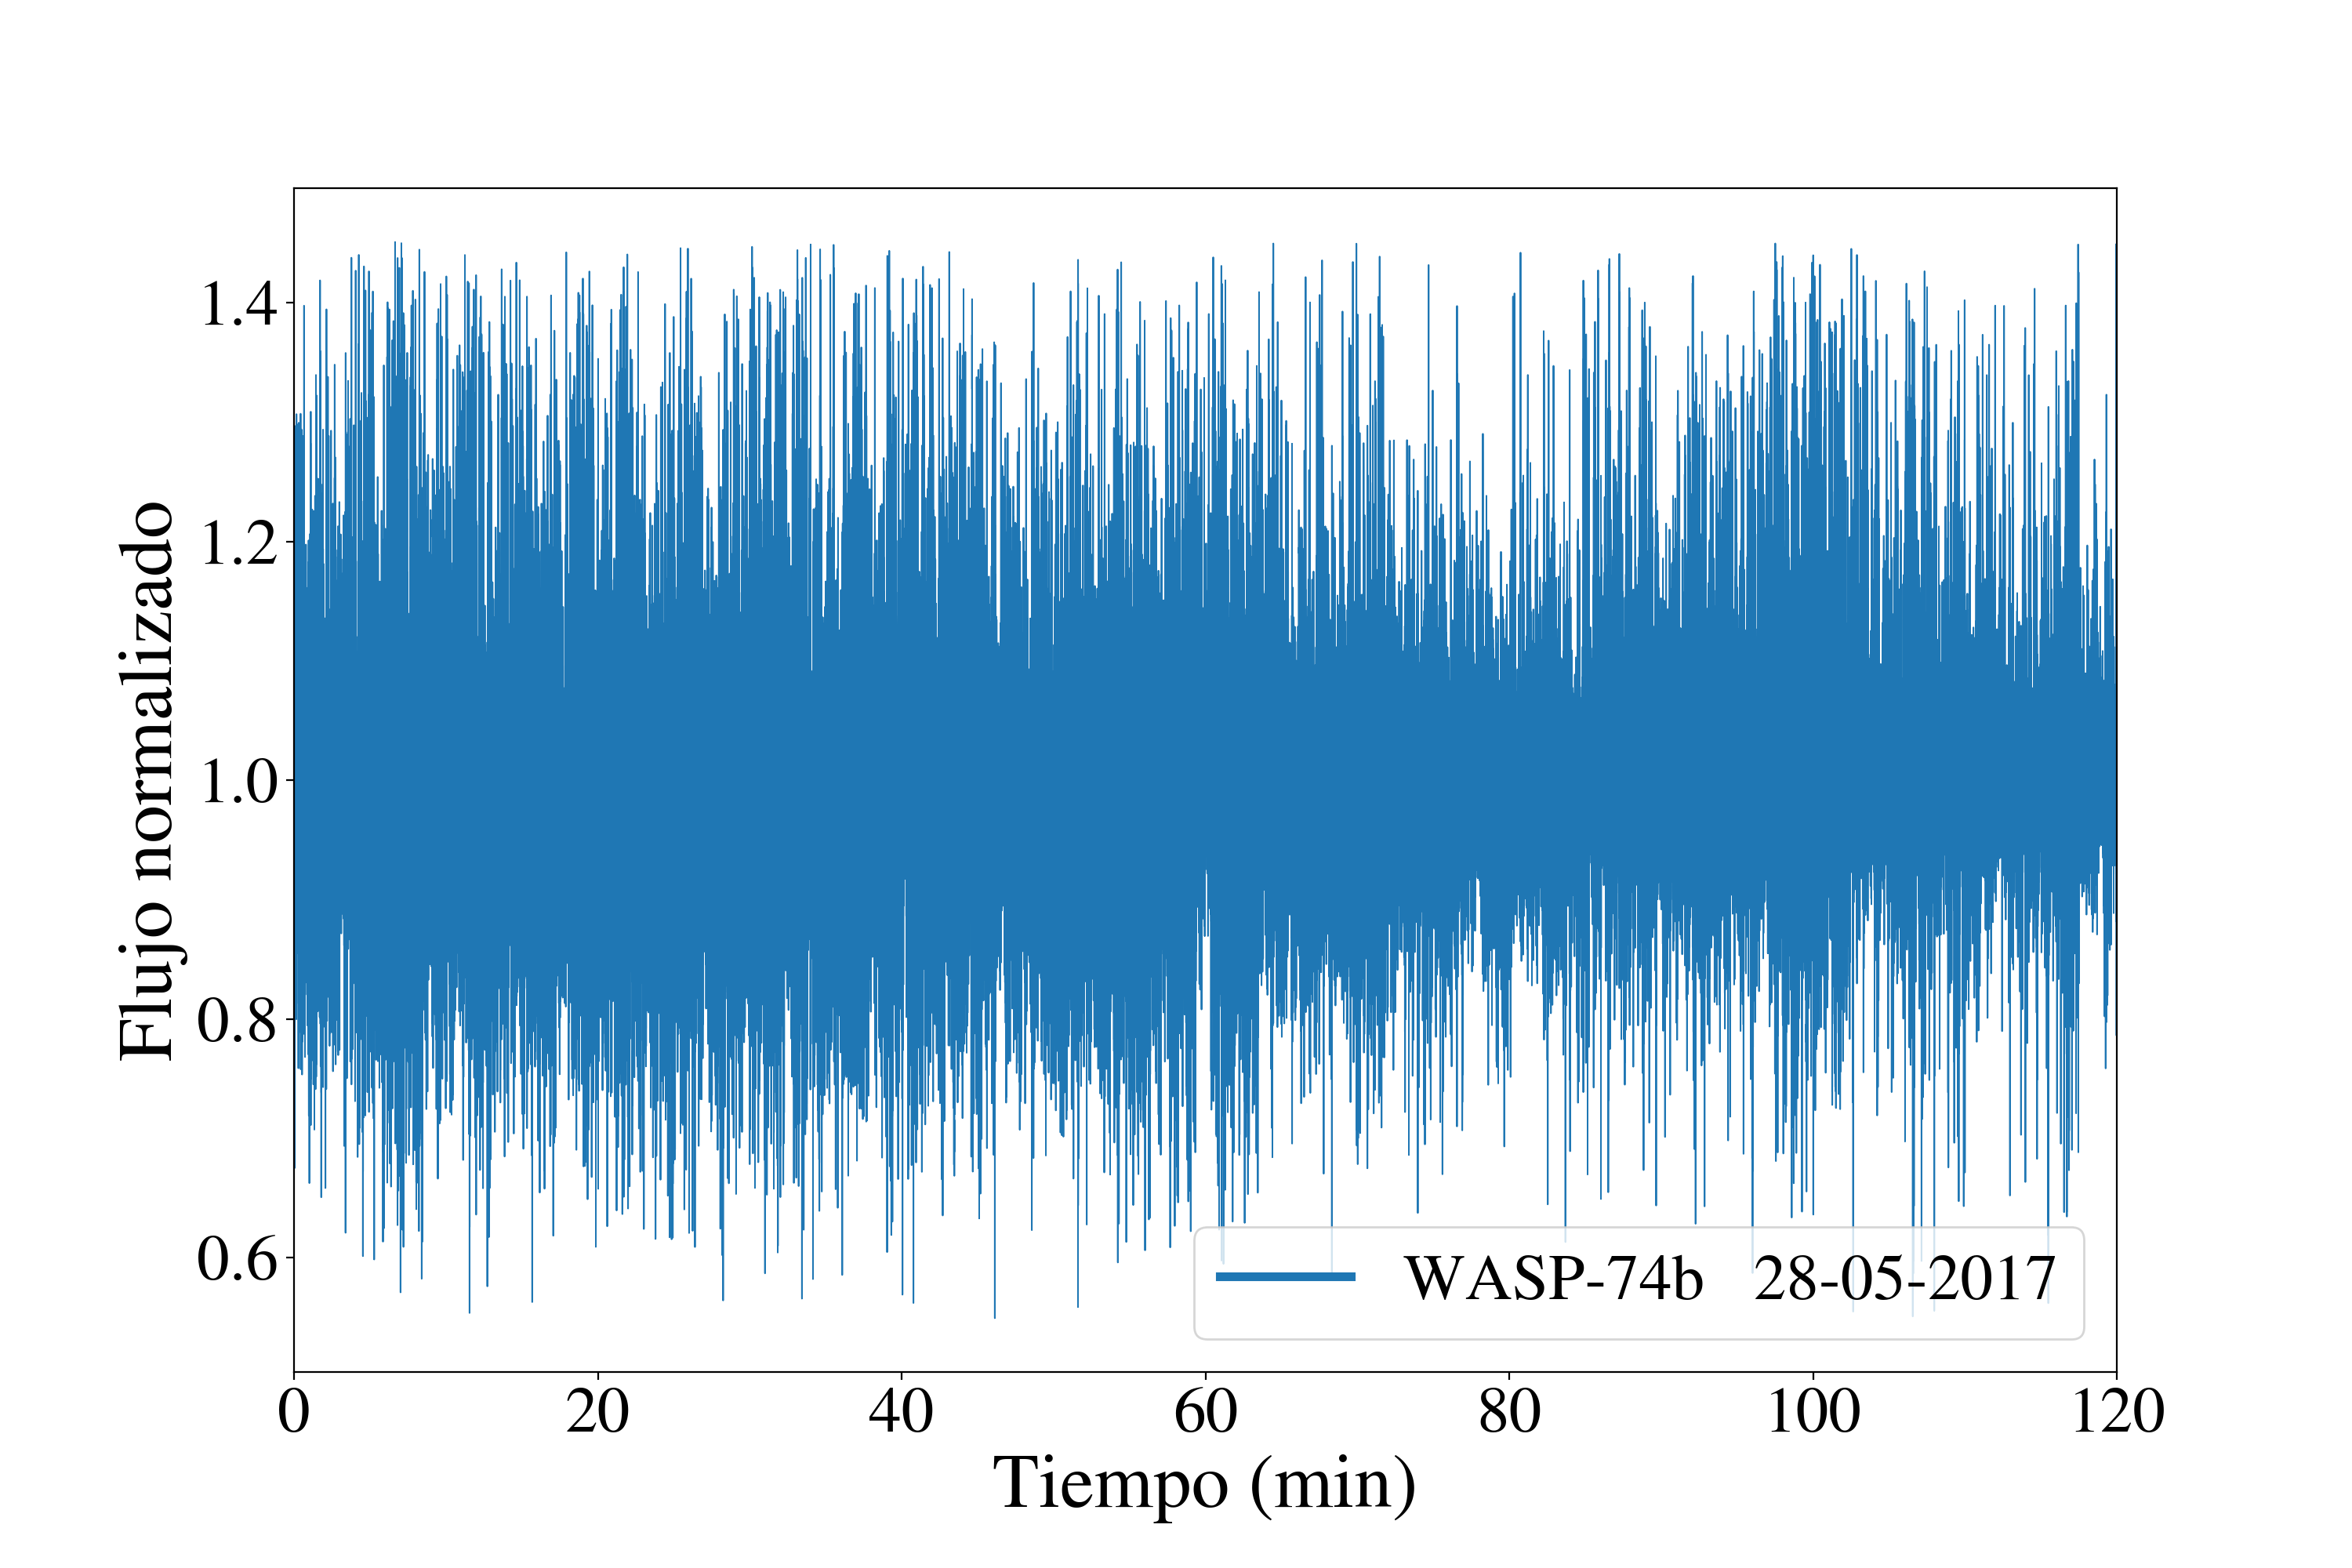
\includegraphics[max size={\textwidth}{0.7\textheight}]{./figures/curva_luz_wasp.png}
   \caption{Fig. 3.4. Curva de luz de WASP-74b, calculada mediante fotometría diferencial usando APPHi.}
    \label{fig:3.4_wasp-74b-curva}
\end{figure}

Esta misma distribución se encontró en diferentes curvas de luz, por lo que se ajustó el modelo \textcolor{red}{ Cual es este modelo??? (3.2)} a las distribuciónes temporales de las curvas de luz. 

\begin{equation}
  m(t)= A_{1}e^{-\dfrac{(t-\mu_{1})^{2}}{2\sigma_{1}^{2}}} + A_{2}e^{-\dfrac{(t-\mu_{2})^{2}}{2\sigma_{2}^{2}}} = G_{1}(t)+G_{2}(t);
\end{equation}
\textcolor{red}{por favor explica esta ecuación y etiquetala correctamente}


El resultado del ajuste de $m(t)$ al histograma de la curva de WASP-74b se muestra en al Figura 3.5.

\begin{figure}[H]
  \centering
    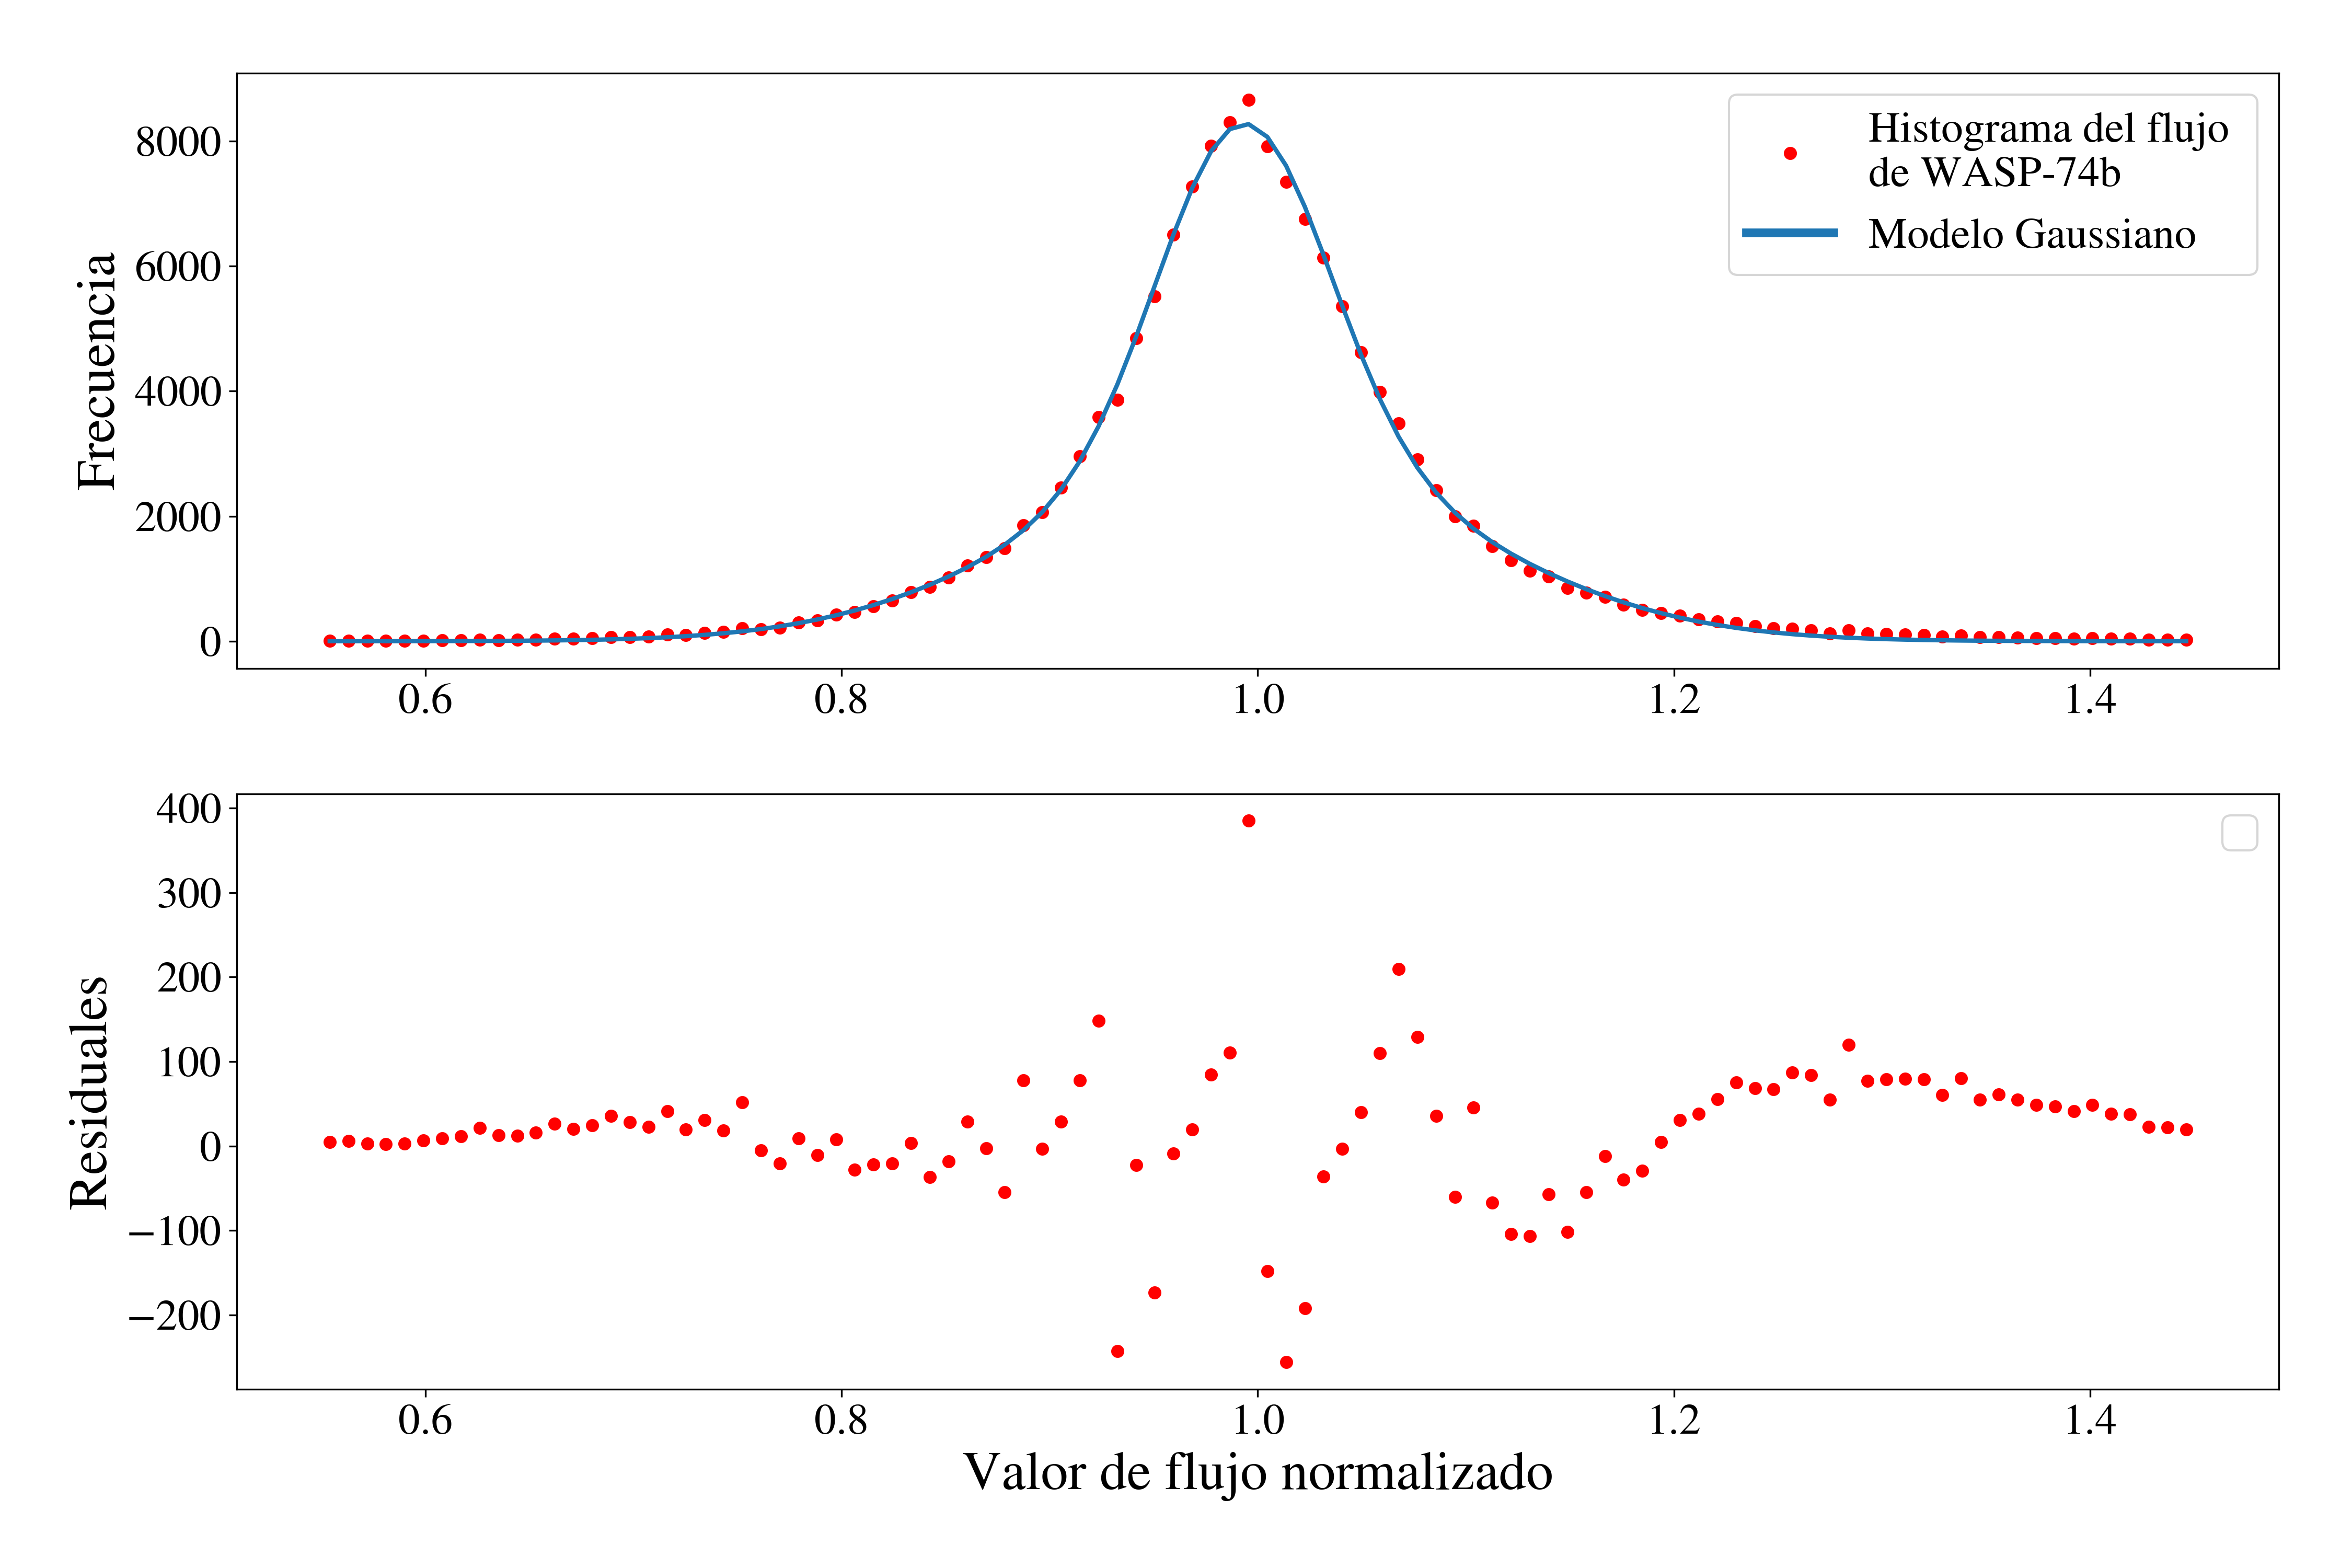
\includegraphics[max size={\textwidth}{0.7\textheight}]{./figures/ajuste_modelo_gaussiano.png}
   \caption{Fig. 3.5. Arriba: Los puntos rojos son la distribución temporal de la curva de luz de WASP-74b. La linea azul sólida, es $m(t)$ resultado de un ajuste no lineal utilizando el algoritmo de Levenberg-Marquardt. Abajo: se aprecia los residuales de la diferencia entre la distribución y el modelo.}
    \label{fig:3.5_wasp-74b-ajuste_residuales}
\end{figure}

La contribución de cada componente $m(t)$ se aprecia en la Figura 3.6. De este gráfico podemos intuir que existen 2 fenómenos \textcolor{red}{Al menos hay que mencionar cuales son esos dos fenómenos} que contribuyen al ruido final en la curva de luz, sin embargo, la fuente de estas componentes no es de interés para los propósitos de este trabajo. 

\begin{figure}[H]
  \centering
    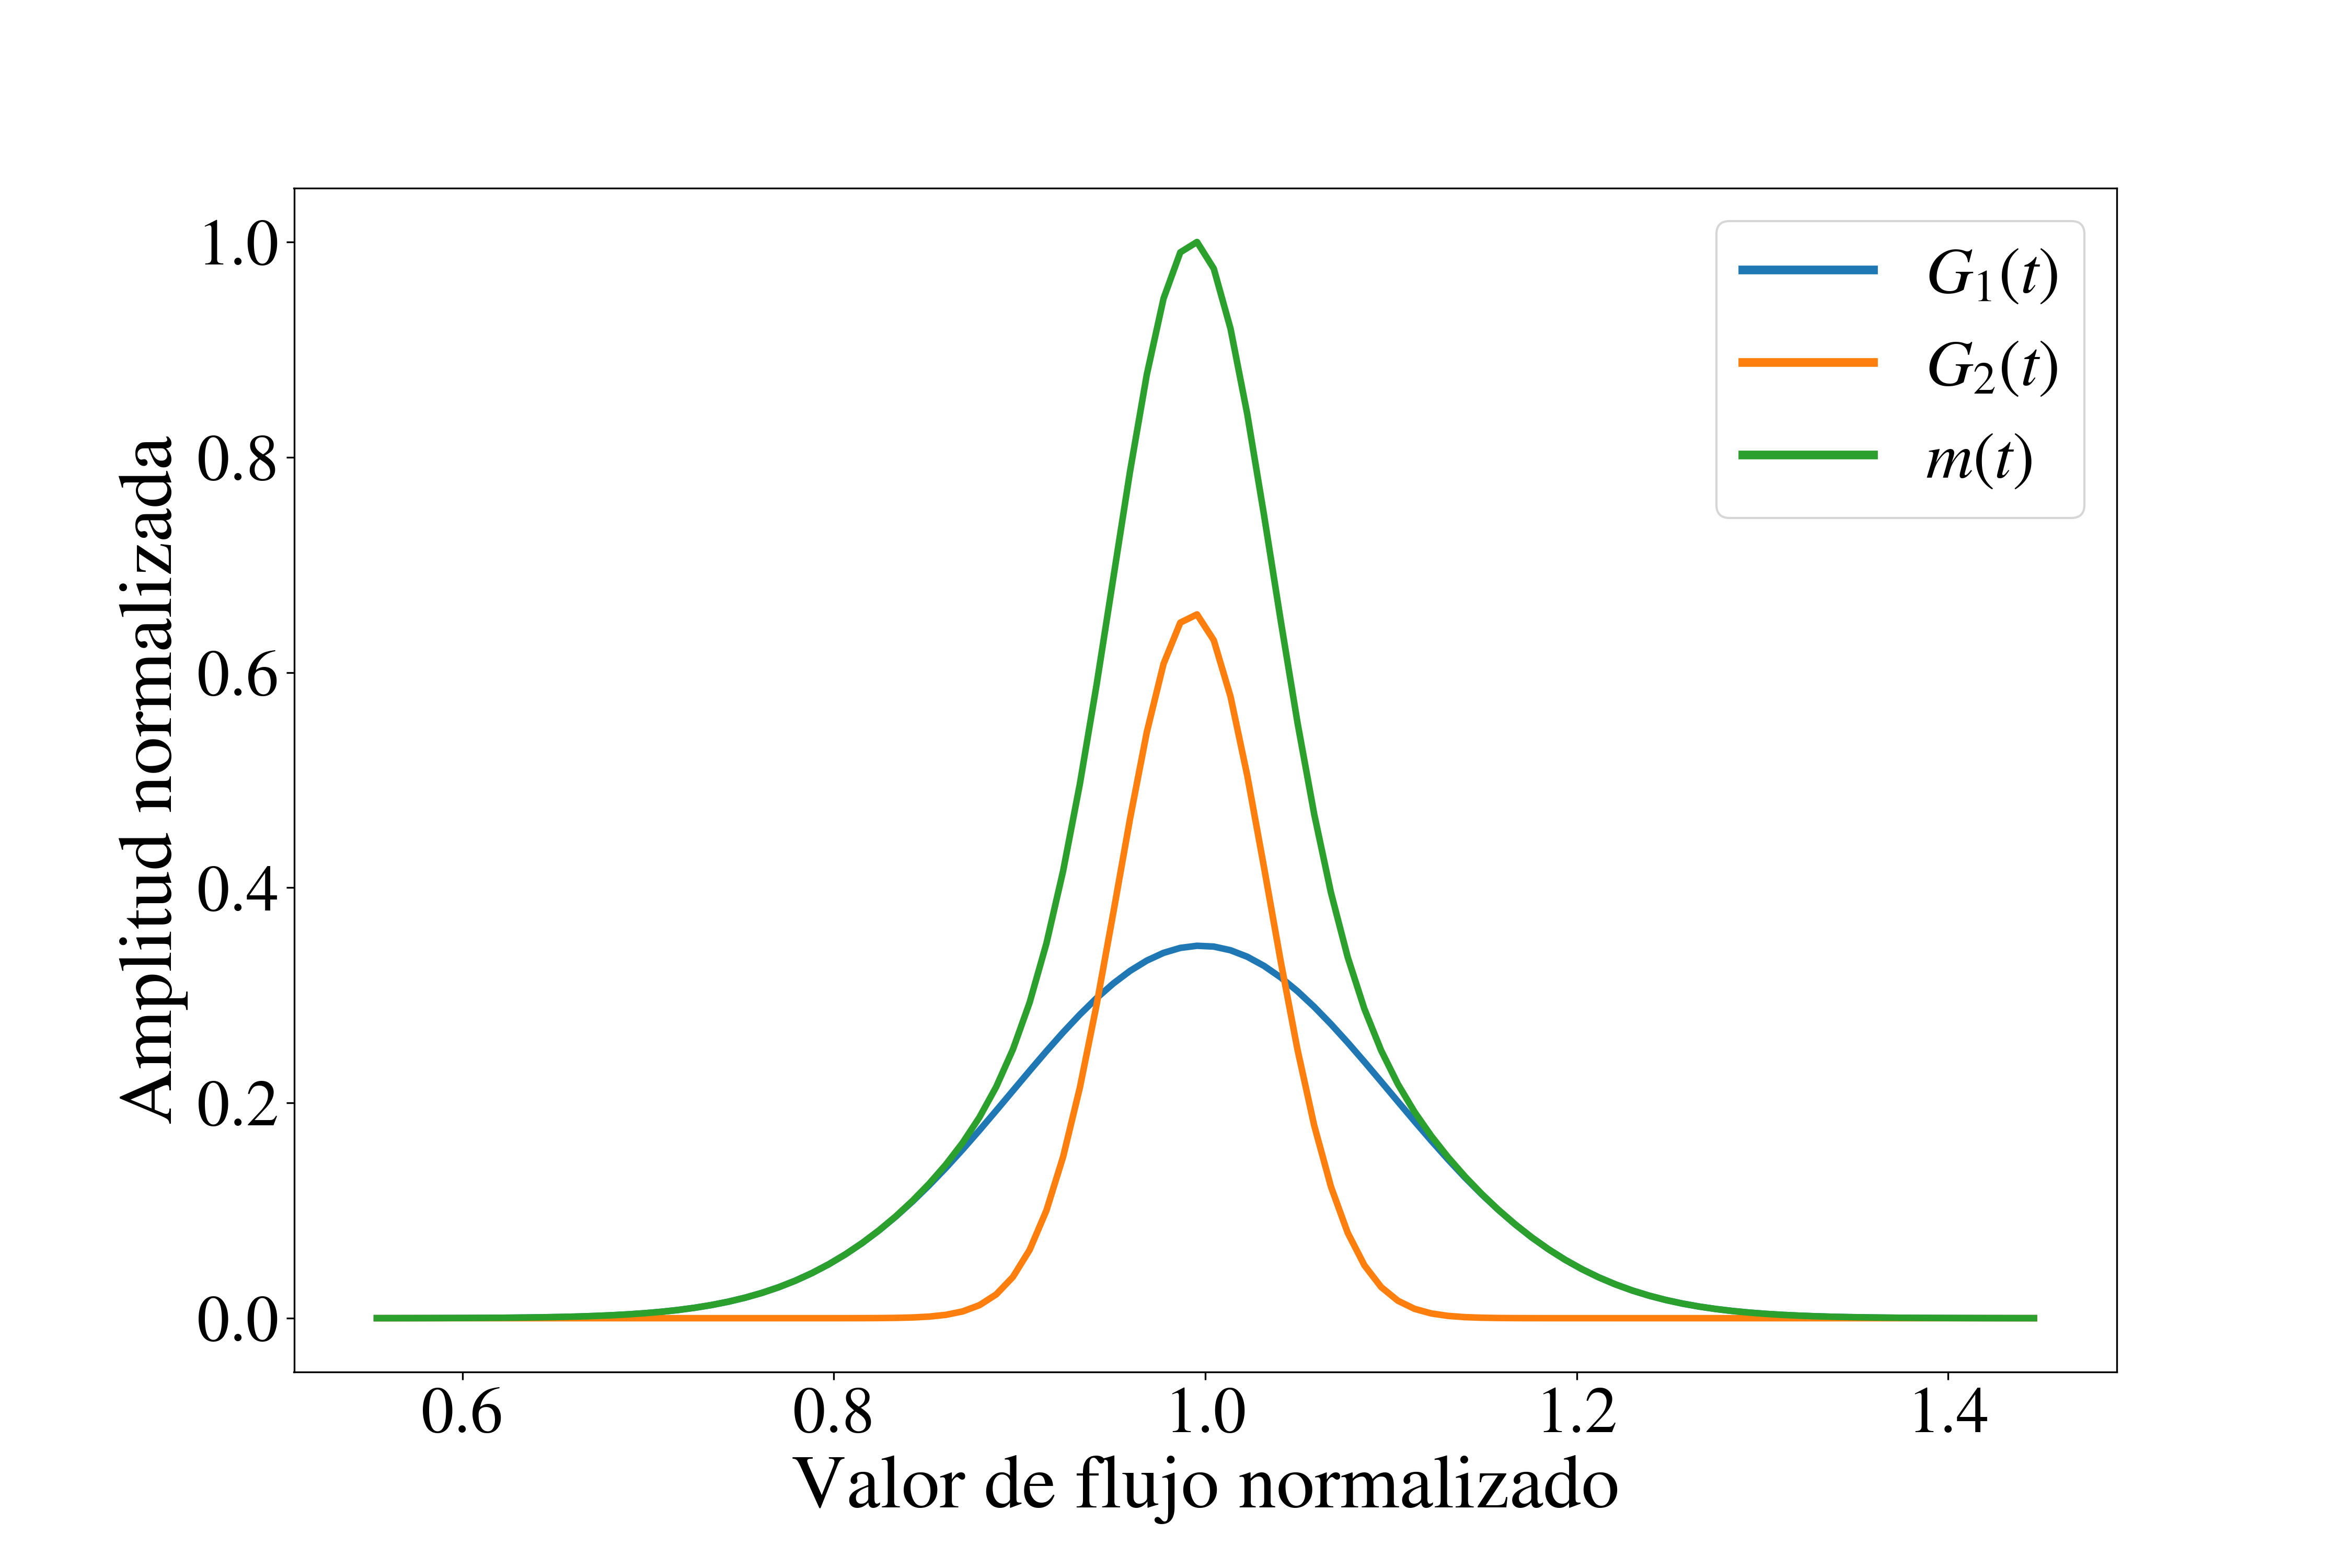
\includegraphics[max size={\textwidth}{0.7\textheight}]{./figures/componentes_gaussianas.png}
   \caption{Fig. 3.6. Se muestra la contribución de las componentes $G_{1}$ y $G_{2}$ y la suma $m(t)$.}
    \label{fig:3.6_wasp-74b-curva}
\end{figure}

Ajustando $m(t)$ a todas las curvas de luz, se encontraron restricciones para el momento en que estemos modelando el ruido (véase III.2.3).

\subsection*{III.2.2 Espectro de frecuencias del ruido}
\addcontentsline{toc}{subsection}{III.2.1 Espectro de frecuencias del ruido}

El ruido blanco como el de la Figura 3.3 tiene un espectro de frecuencias plano, incluso la suma de 2 componentes de ruido gaussiano sigue teniendo un espectro de potencias plano como se aprecia en la Figura 3.7

\begin{figure}[H]
  \centering
    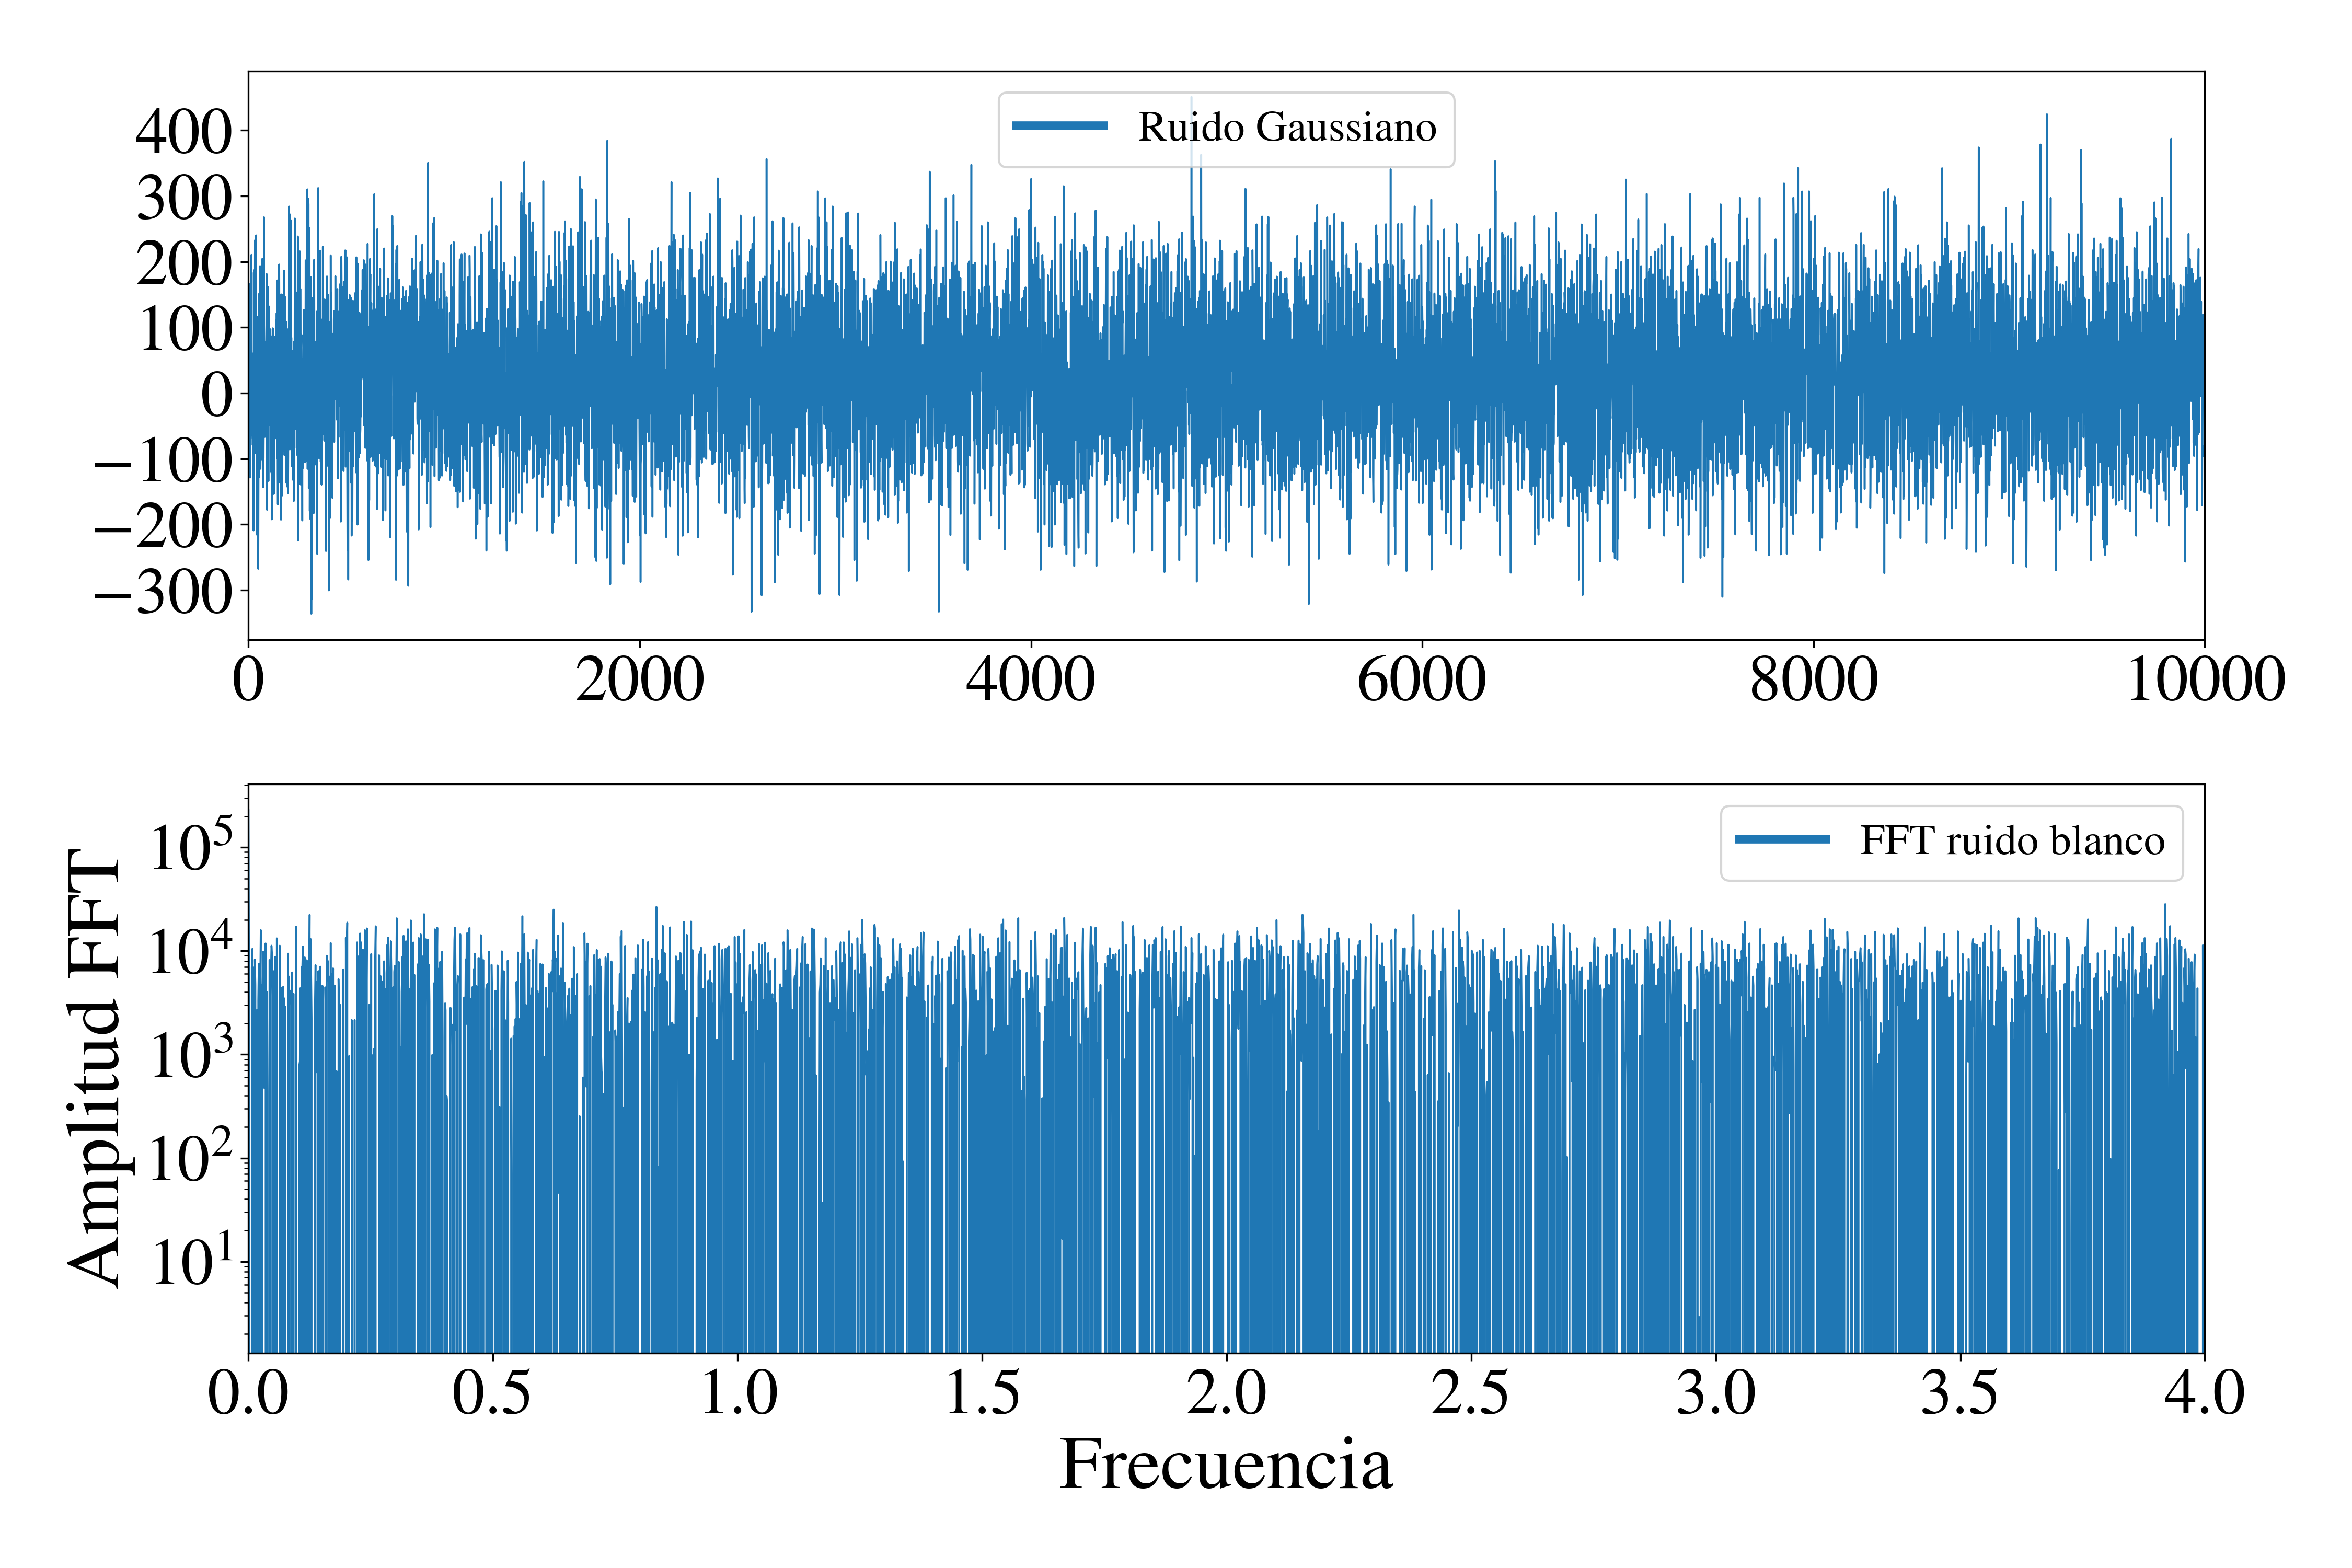
\includegraphics[max size={\textwidth}{0.7\textheight}]{./figures/ejemplo_espectro_gauss.png}
   \caption{Fig. 3.7. Arriba: Se muestra una curva de ruido blanco con dos componentes $G_{1}$ y $G_{2}$. Abajo: El espectro de frecuencias de la curva de luz, el cual permanece blanco sin importar el número de componentes gaussianas.}
    \label{fig:3.7_wasp-74b-curva}
\end{figure}

Sin embargo, al analizar las curvas de luz se encontró que un espectro de frecuencias plano, es solo un caso muy párticular, solo 2 de las 12 mejores curvas de luz presentaron un espectro plano. Todas las otras curvas tienen una significativa componente de bajas frecuencias, así como una ligera pendiente negativa, disminuyendo hacia las frecuencias altas como se aprecia en la figura \ref{fig_2_8_fourier}.\textcolor{red}{esa figura no existe}

Entonces si queremos simular ruido, que posea características que se aprecian en una curva de luz real, necesitamos más que una simple distribución gaussiana. Por lo que esta distribución temporal es solo el punto de partida para generar un ruido sintético. 

Para añadir estas contribuciones de baja frecuencia, se modeló una envolvente exponencial de la forma:

\begin{equation}
  \displaystyle E(f)= C + a_{1}e^{-\dfrac{f}{b_{1}}} + a_{2}e^{-\dfrac{f}{b_{2}}};
\end{equation}

utilizando esta envolvente se altera el espectro de frecuencias de acuerdo a lo observado en las curvas de luz. De manera similar a la metodología implementada para las distribuciónes temporales, se calcularon los parámetros de $E(f)$ para todas las curvas de luz y se obtuvieron restricciones para la posterior simulación de ruido sintético.
\textcolor{red}{otra vez, por favor explica la ecuacion}
\begin{figure}[H]
  \centering
    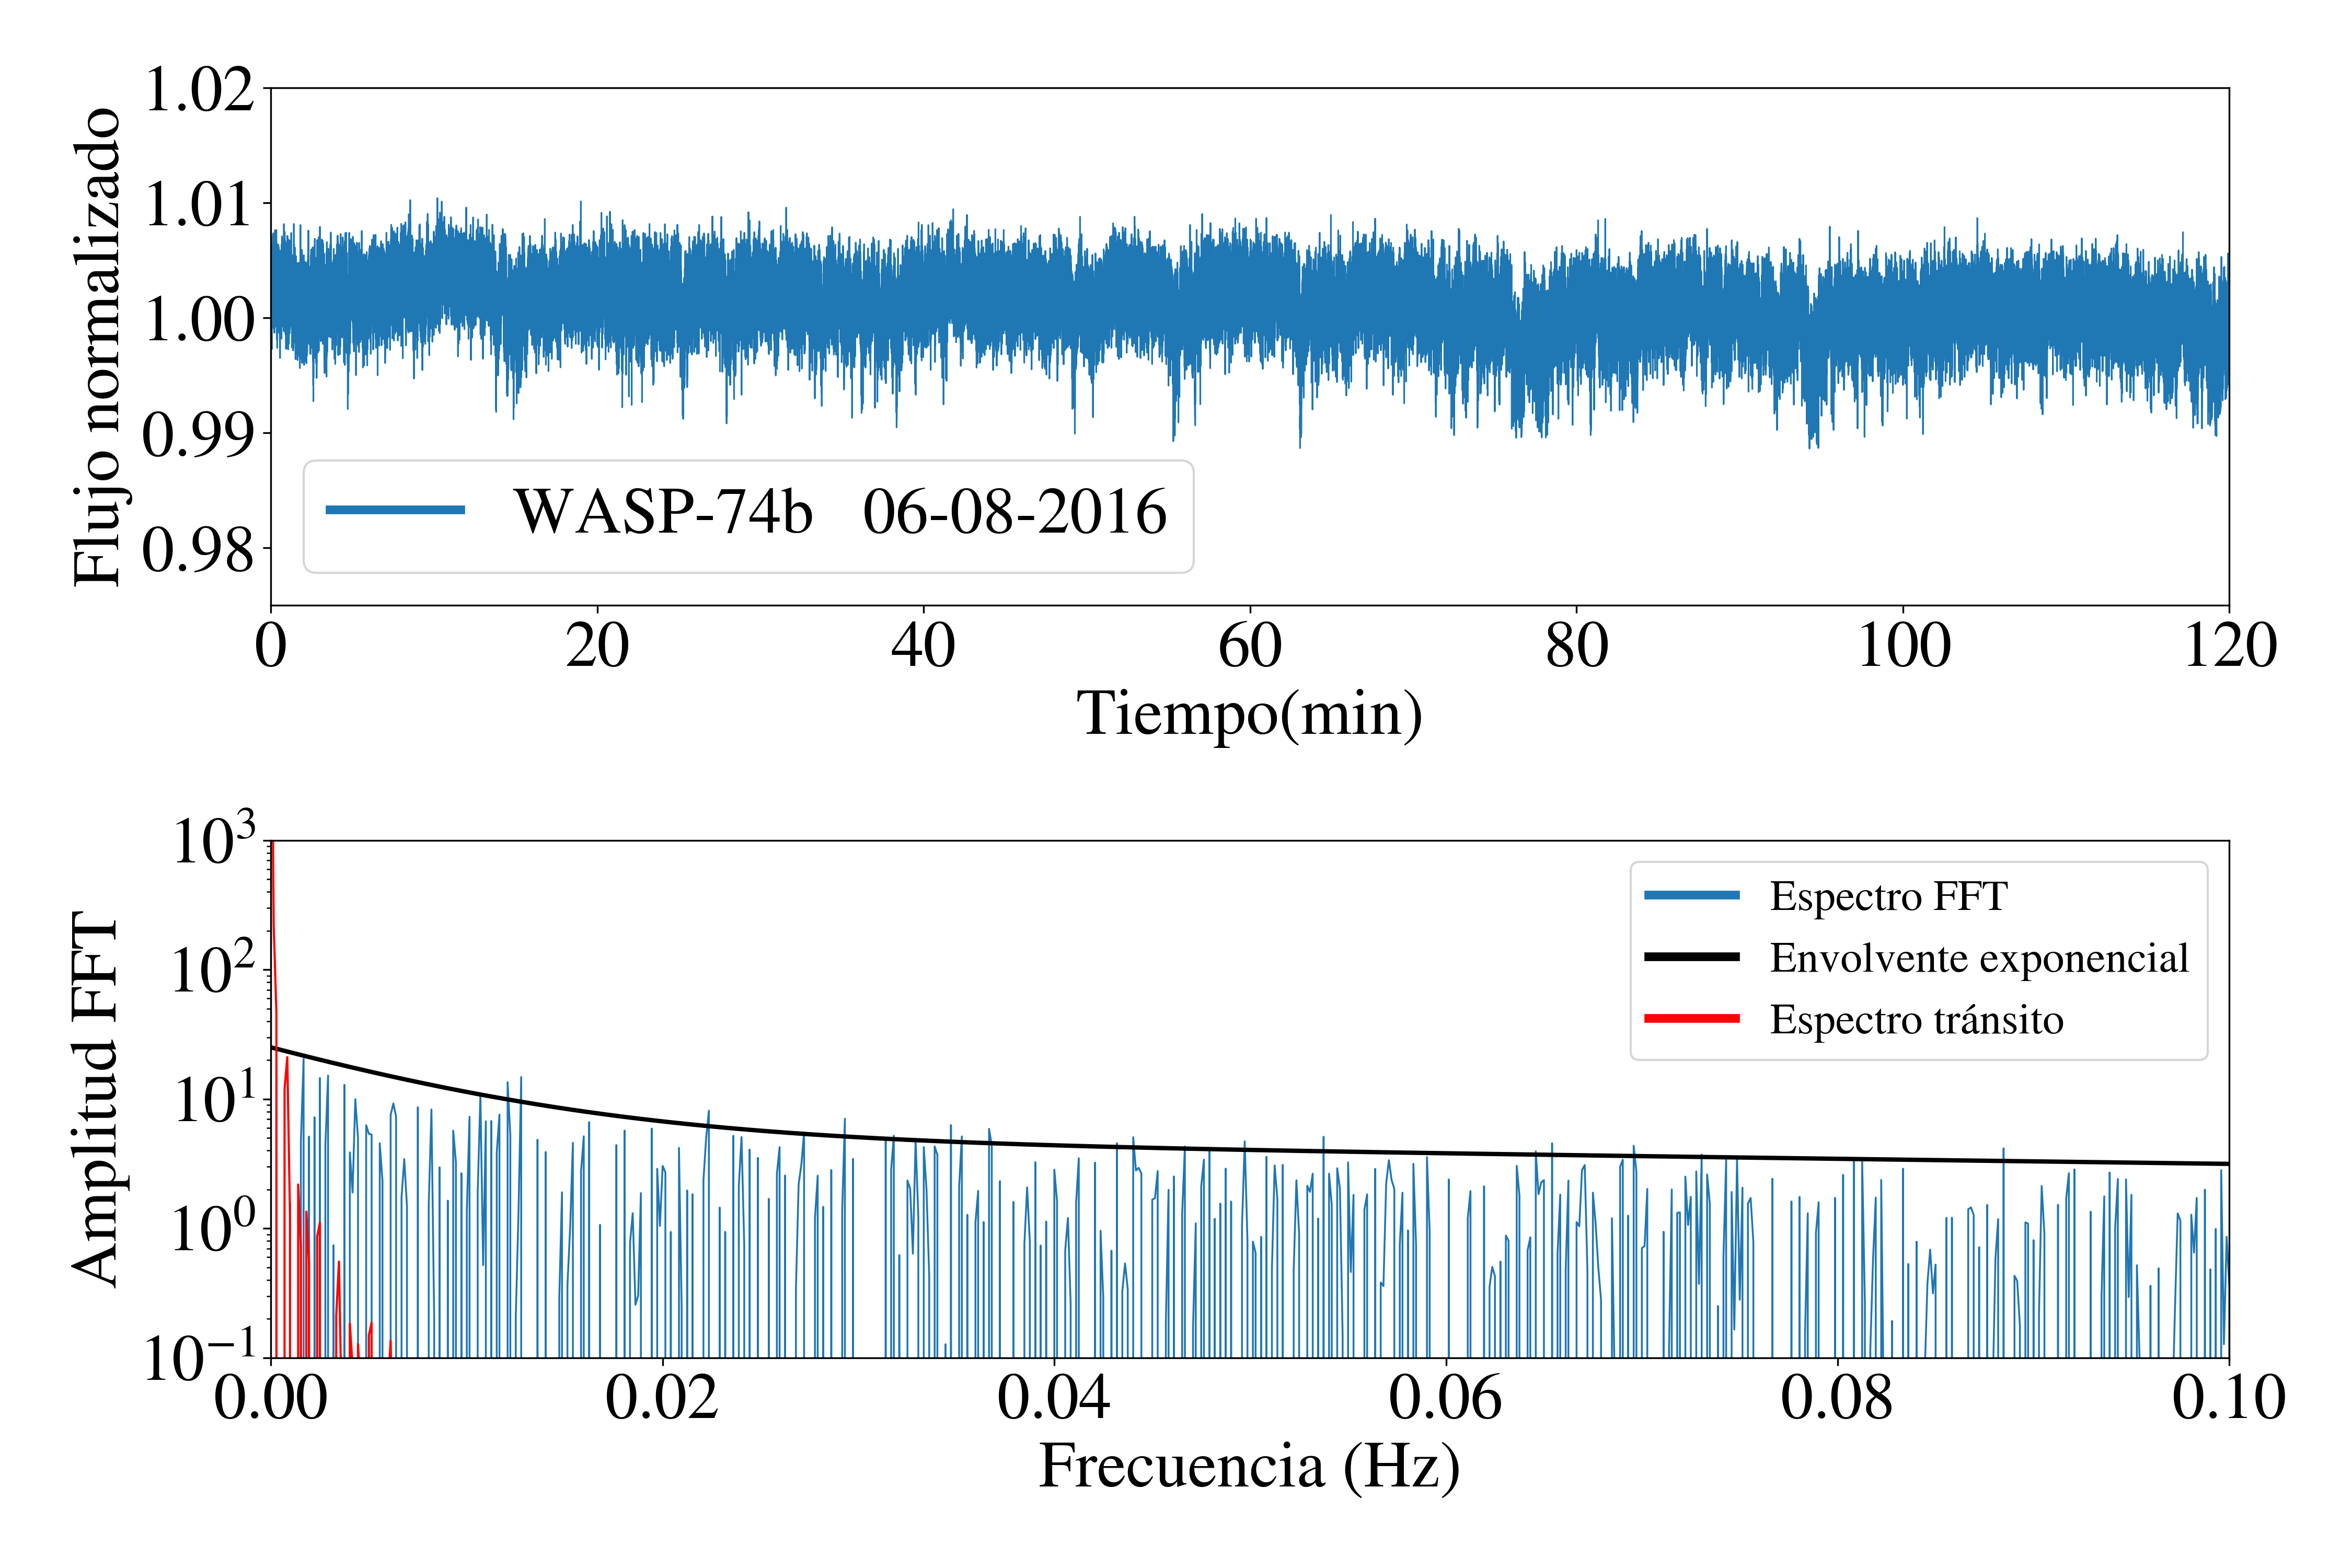
\includegraphics[max size={\textwidth}{0.7\textheight}]{./figures/curva_ajuste_espectro.png}
   \caption{Fig. 3.7. Arriba: Se muestra una curva de luz de WASP-74b. Abajo: La zona de bajas frecuencias del espectro de la curva de luz, la linea roja es el ajuste de la envolvente exponencial $E(f)$ del espectro.}
    \label{fig:3.7_wasp-74b-curva}
\end{figure}
\textcolor{red}{explicar la figura}
\subsection*{III.2.3 Simulación de ruido}
\addcontentsline{toc}{subsection}{III.2.3 Simulación de ruido}

Utilizando los resultados obtenidos siguiendo la metodología de las secciónes anteriores (III.2.2 y III.2.3) se implementó un algoritmo para generar ruido con características que podemos observar y medir en curvas de luz reales.

Primeramente, para simular un ruido $R(t)$ \textcolor{red}{tienes que poner la ecuación que relacione R(t)}, dada una función de distribución $m(t)$, calculamos la función de distribución acumulativa:

\begin{equation}
  \displaystyle M(t)= \int m(t)dt;
\end{equation}

\noindent y después normalizamos $M(t)$:

\begin{equation}
  \displaystyle M_{norm}(t)= \dfrac{M(t)}{\mbox{MAX}(M(t))};
\end{equation}

Para generar el vector de ruido, se realiza un muestreo de puntos aleatorios $t_{i}$ con distribución uniforme $\mathcal{U}(a,b)$, evaluados en la función inversa de la distribución acumulada normalizada, denotada como: $M^{-1}_{norm}$. Resumiendo, a continuación se muestran  los pasos a seguir:

\begin{itemize}
  \item Elegir la distribución del ruido deseado, (en este caso usamos $m(t)$ (3.17)).
  \item Calcular la función de distribución acumulada $M(t)$ (3.19).
  \item Normalizar $M(t)$ (3.20).
  \item Encontrar la función inversa de $M_{norm}(t)$.
  \item Evaluar $t_{i}$ con $i=1,..,N$ puntos en $M^{-1}_{norm}(t_{i})$
\end{itemize}

El resultado es una serie de tiempo $R(t)$ normalizada, de longitud $N$ con distribución $m(t)$. Algo que no se mencionó fueron los valores de los parámetros $(A_{1},\mu_{1},\sigma_{1},A_{2},\mu_{2},\sigma_{2})$ \textcolor{red}{explicar que son cada uno de esos parámetros} de la función de distribución $m(t)$. Esto es porque pueden ser elegidos de manera arbitraria, dado que podemos cambiar la SNR de la serie de tiempo simplemente con: $R(t)*\sigma$. Para una curva normalizada $(\mu=1)$ la SNR es igual a $\sigma^{-1}$. Con esto podemos elegir la SNR que se necesite.

Sin embargo, como mencionamos anteriormente, necesitamos una serie de tiempo de ruido simulado $R(t)$ con un espectro no plano. Para esto, calculamos la FFT de $R(t)$ y multiplicamos su espectro de frecuencias por una envolvente $E(f)$. El desglose detallado de los pasos a seguir es el siguiente:

\begin{itemize}
  \item Calcular la FFT de $R(t)$ la cual denotaremos como $\mathcal{R}(f)$.
  \item Generar de manera aleatoria los parámetros $(C,a_{1},b_{1},a_{2},b_{2})$ distribuidos de manera uniforme dentro de los límites.
  \item Generar una envolvente evaluando los parámetros del paso anterior $E((C,a_{1},b_{1},a_{2},b_{2}),f)$.
  \item Multiplicar $\mathcal{R}(f)*E(f)$.
  \item Calcular la FFT inversa para regresar al dominio del tiempo.
  \item Normalizar la nueva $R(t)$.
  \item Elegir $\sigma$ para obtener la SNR deseada.
\end{itemize}

Esto resulta en una serie de tiempo, con $SNR=\sigma^{-1}$, con algunos ruidos sistemáticos aleatorios. En la figura 3.8 se muestra una comparación de el espectro de frecuencias de la curva de luz de WASP-74b comparado con el ruido simulado, usando la envolvente $E(f)$ calculada de su espectro.

\begin{figure}[H]
  \centering
    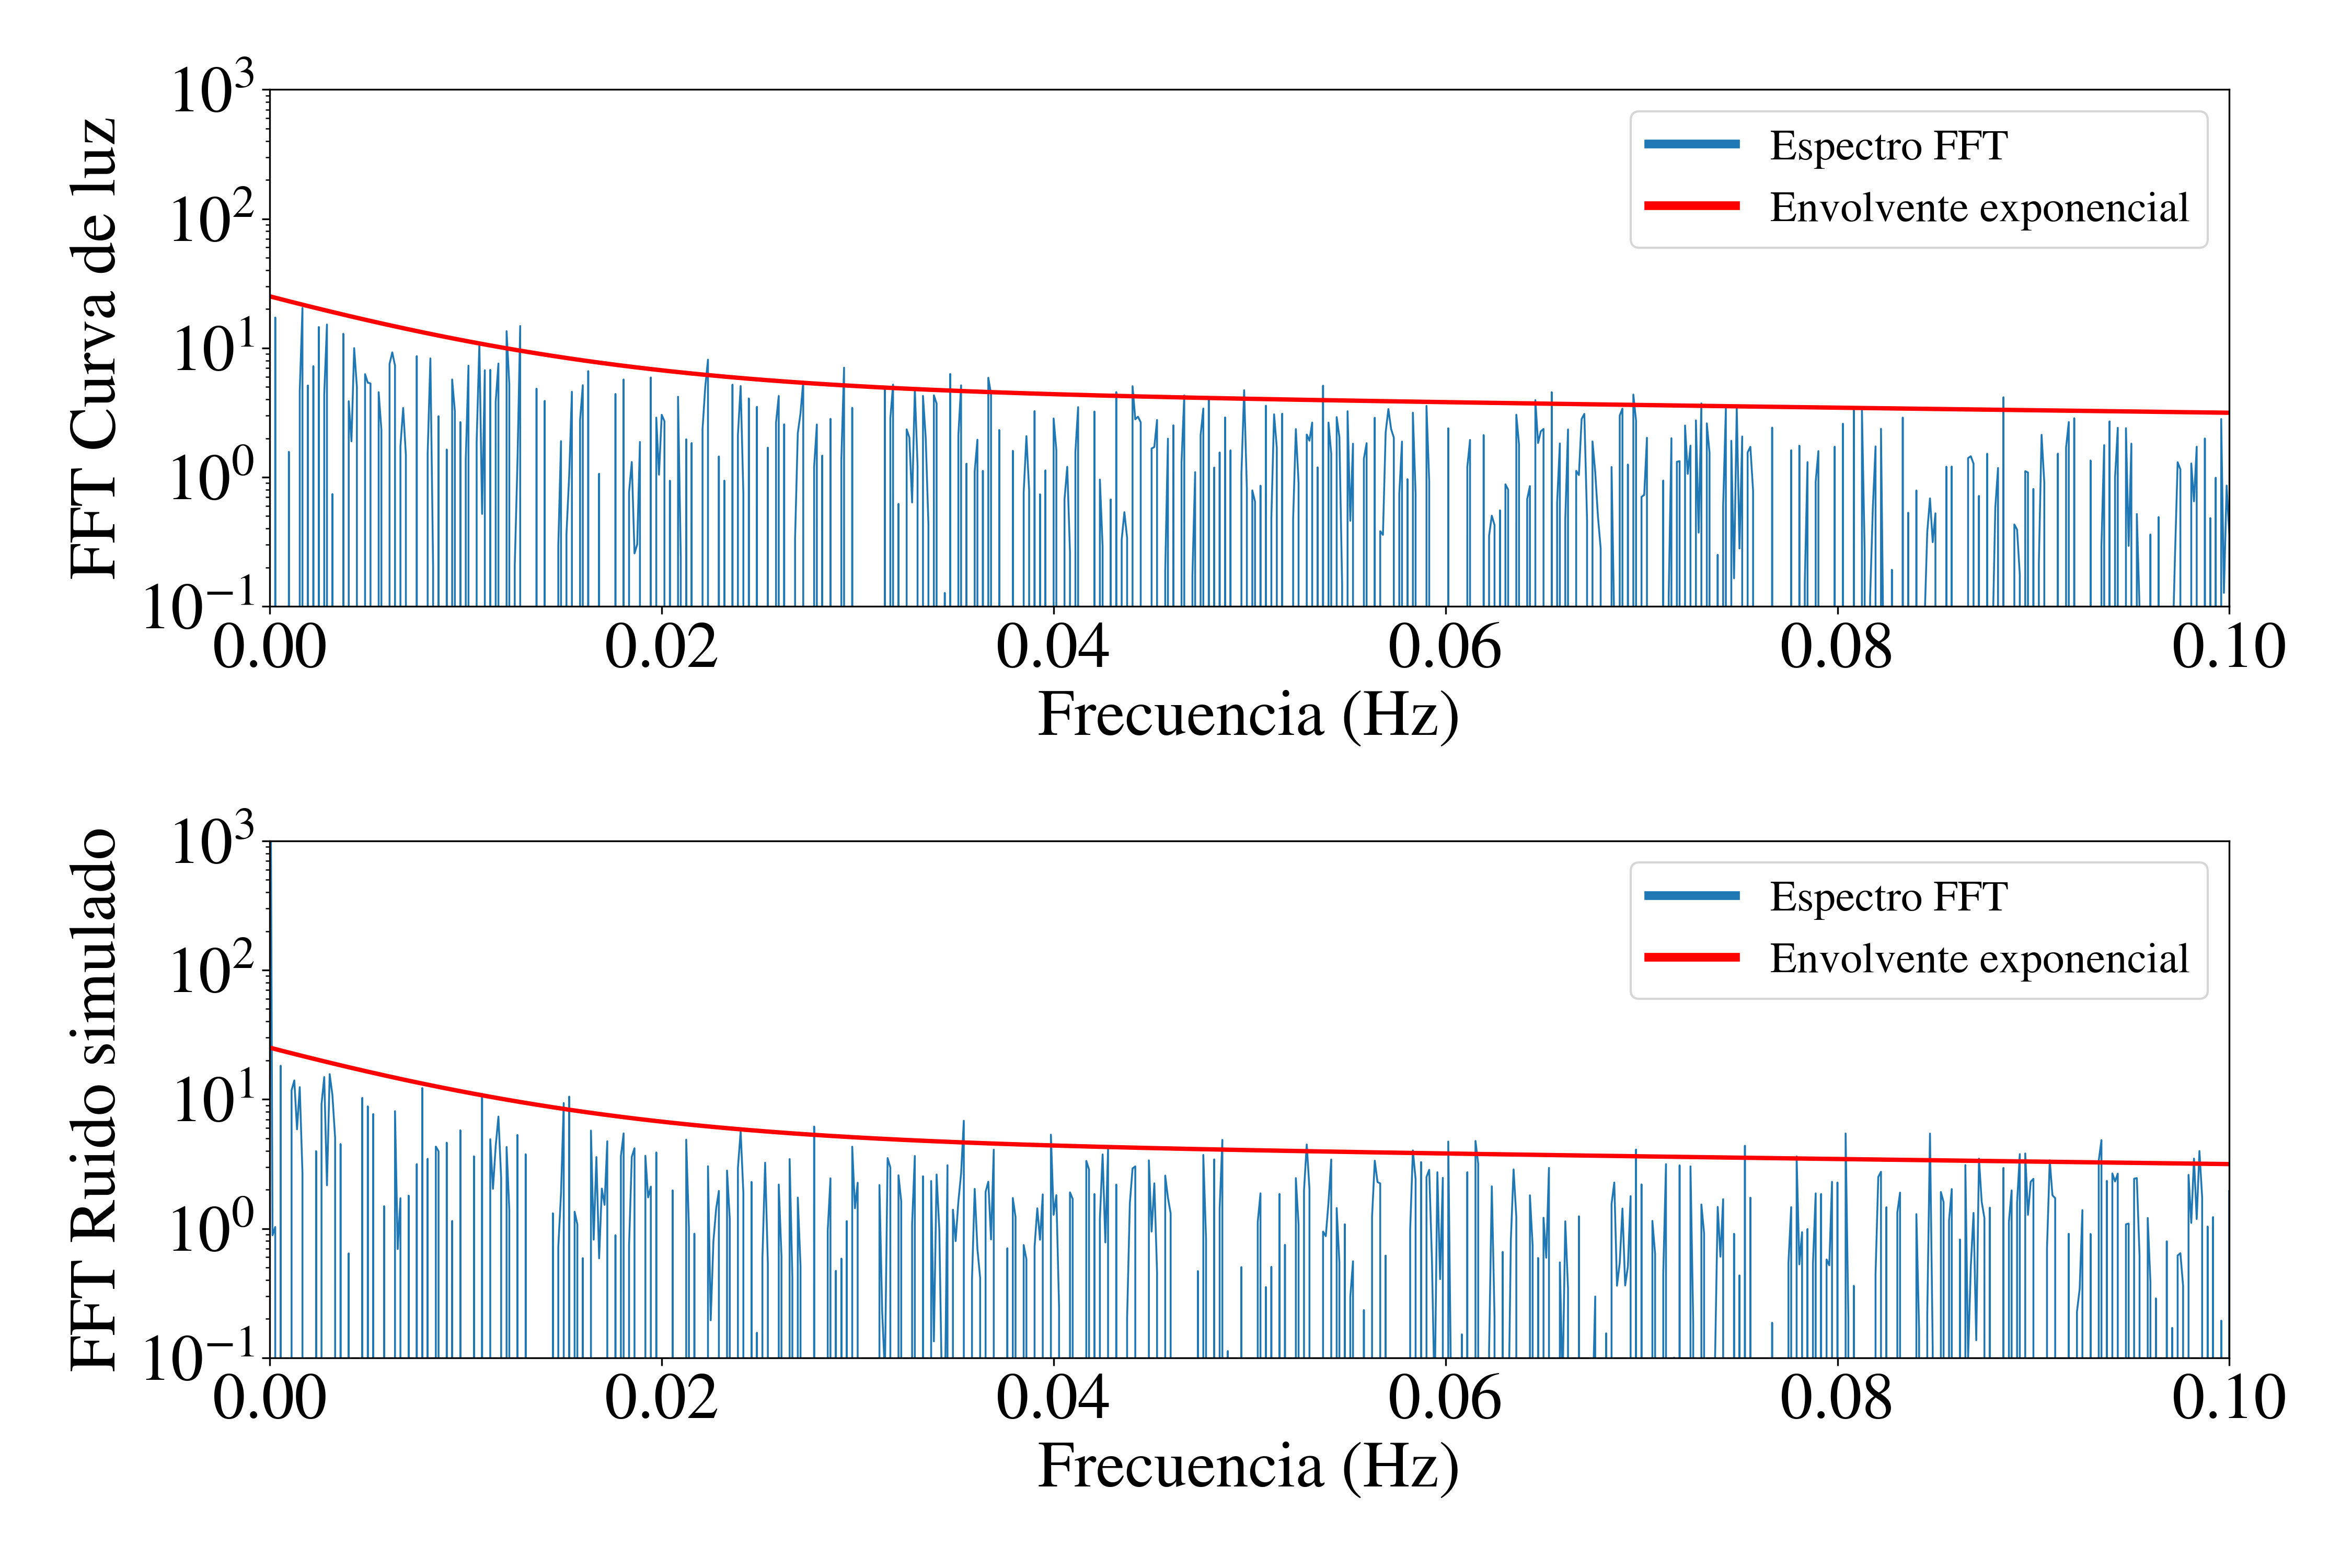
\includegraphics[max size={\textwidth}{0.7\textheight}]{./figures/comparacion_espectros.png}
   \caption{Fig. 3.8. Arriba: Se muestra la FFT de la curva de luz de WASP-74b. Abajo: El espectro de frecuencias de la serie de tiempo $R(t)$ generada utilizando la metodología planteada en esta sección. Ambas gráficas son un acercamiento a la zona de bajas frecuencias para mejorar la visualización. La linea roja es la misma envolvente exponencial $E(f)$ para ambos espectros.}
    \label{fig:3.8_comp_espectros}
\end{figure}

Utilizando esta metodología, se creó una base de datos de ruidos simulados para asegurar reproducibilidad. Se variaron los parámetros $(C,a_{1},b_{1},a_{2},b_{2})$ de manera uniforme dentro de los intervalos:

\begin{equation}
  \begin{split}
  0.85 \leq C \leq 10 \\
  0 \leq a_{1} \leq 30 \\
  0.02 \leq b_{1} \leq 2.5 \\
  0 \leq a_{2} \leq 150 \\
  0.0029 \leq b_{2} \leq 0.06 \\
  \end{split}
\end{equation}

estos invervalos se calcularon a partir de los espectros de los datos observacionales. Se generaron 100 curvas de ruido por cada valor de SNR. Los valores de SNR utilizados fueron 10, 20, 50, 80 y 100.


\section*{III.3 Simulación de tránsitos de exoplanetas}
\addcontentsline{toc}{section}{III.3 Simulación de tránsitos de exoplanetas}


Como se mencionó anteriormente (sección II.1), la curva de luz de un tránsito de exoplaneta depende de múltiples factores cómo el tamaño de la estrella, el tamaño del planeta, la velocidad orbital del planeta, el ángulo con respecto a la línea de visión etc.

Para la simulación de curvas de luz en este trabajo, se utilizó la paquetería BATMAN (del inglés \textit{BAsic Transit Model cAlculatioN}) desarrollada en \textit{Python} \cite{kreidberg2015batman}. Este algoritmo utiliza el modelo analítico propuesto en \cite{mandel2002analytic}


\subsection*{III.3.1 Descripción y uso de BATMAN}
\addcontentsline{toc}{subsection}{III.3.1 Descripción y uso de BATMAN}

BATMAN es un paquete para \textit{Python}, con el cual se modelan tránsitos de exoplanetas y sus curvas de luz. El código usa extensiones en C para aumentar la velocidad de calculo y esta paralelizado con OpenMP \cite{kreidberg2015batman}. BATMAN puede calcular curvas de luz para cualquier ley de oscurecimiento de limbo radial, usando un nuevo algoritmo de integración que no puede ser calculado analíticamente.

Para utilizar BATMAN, se requiere ingresar los parámetros físicos de los cuáles depende el tránsito, tales como: el periodo orbital $(P)$, el radio del planeta $(R_{p})$ y el semieje mayor $(a)$, ambos en unidades del radio de la estrella anfitriona $(R_{*})$;  la excentricidad de la órbita $(\epsilon)$, la inclinación orbital $(i)$ y la longitud del periastro $(\bar{\omega})$ ambos en grados. Además se puede seleccionar la ley de oscurecimiento radial. En la figura 3.9 se muestra un ejemplo de curvas de luz simuladas con BATMAN. 

\begin{figure}
  \centering
    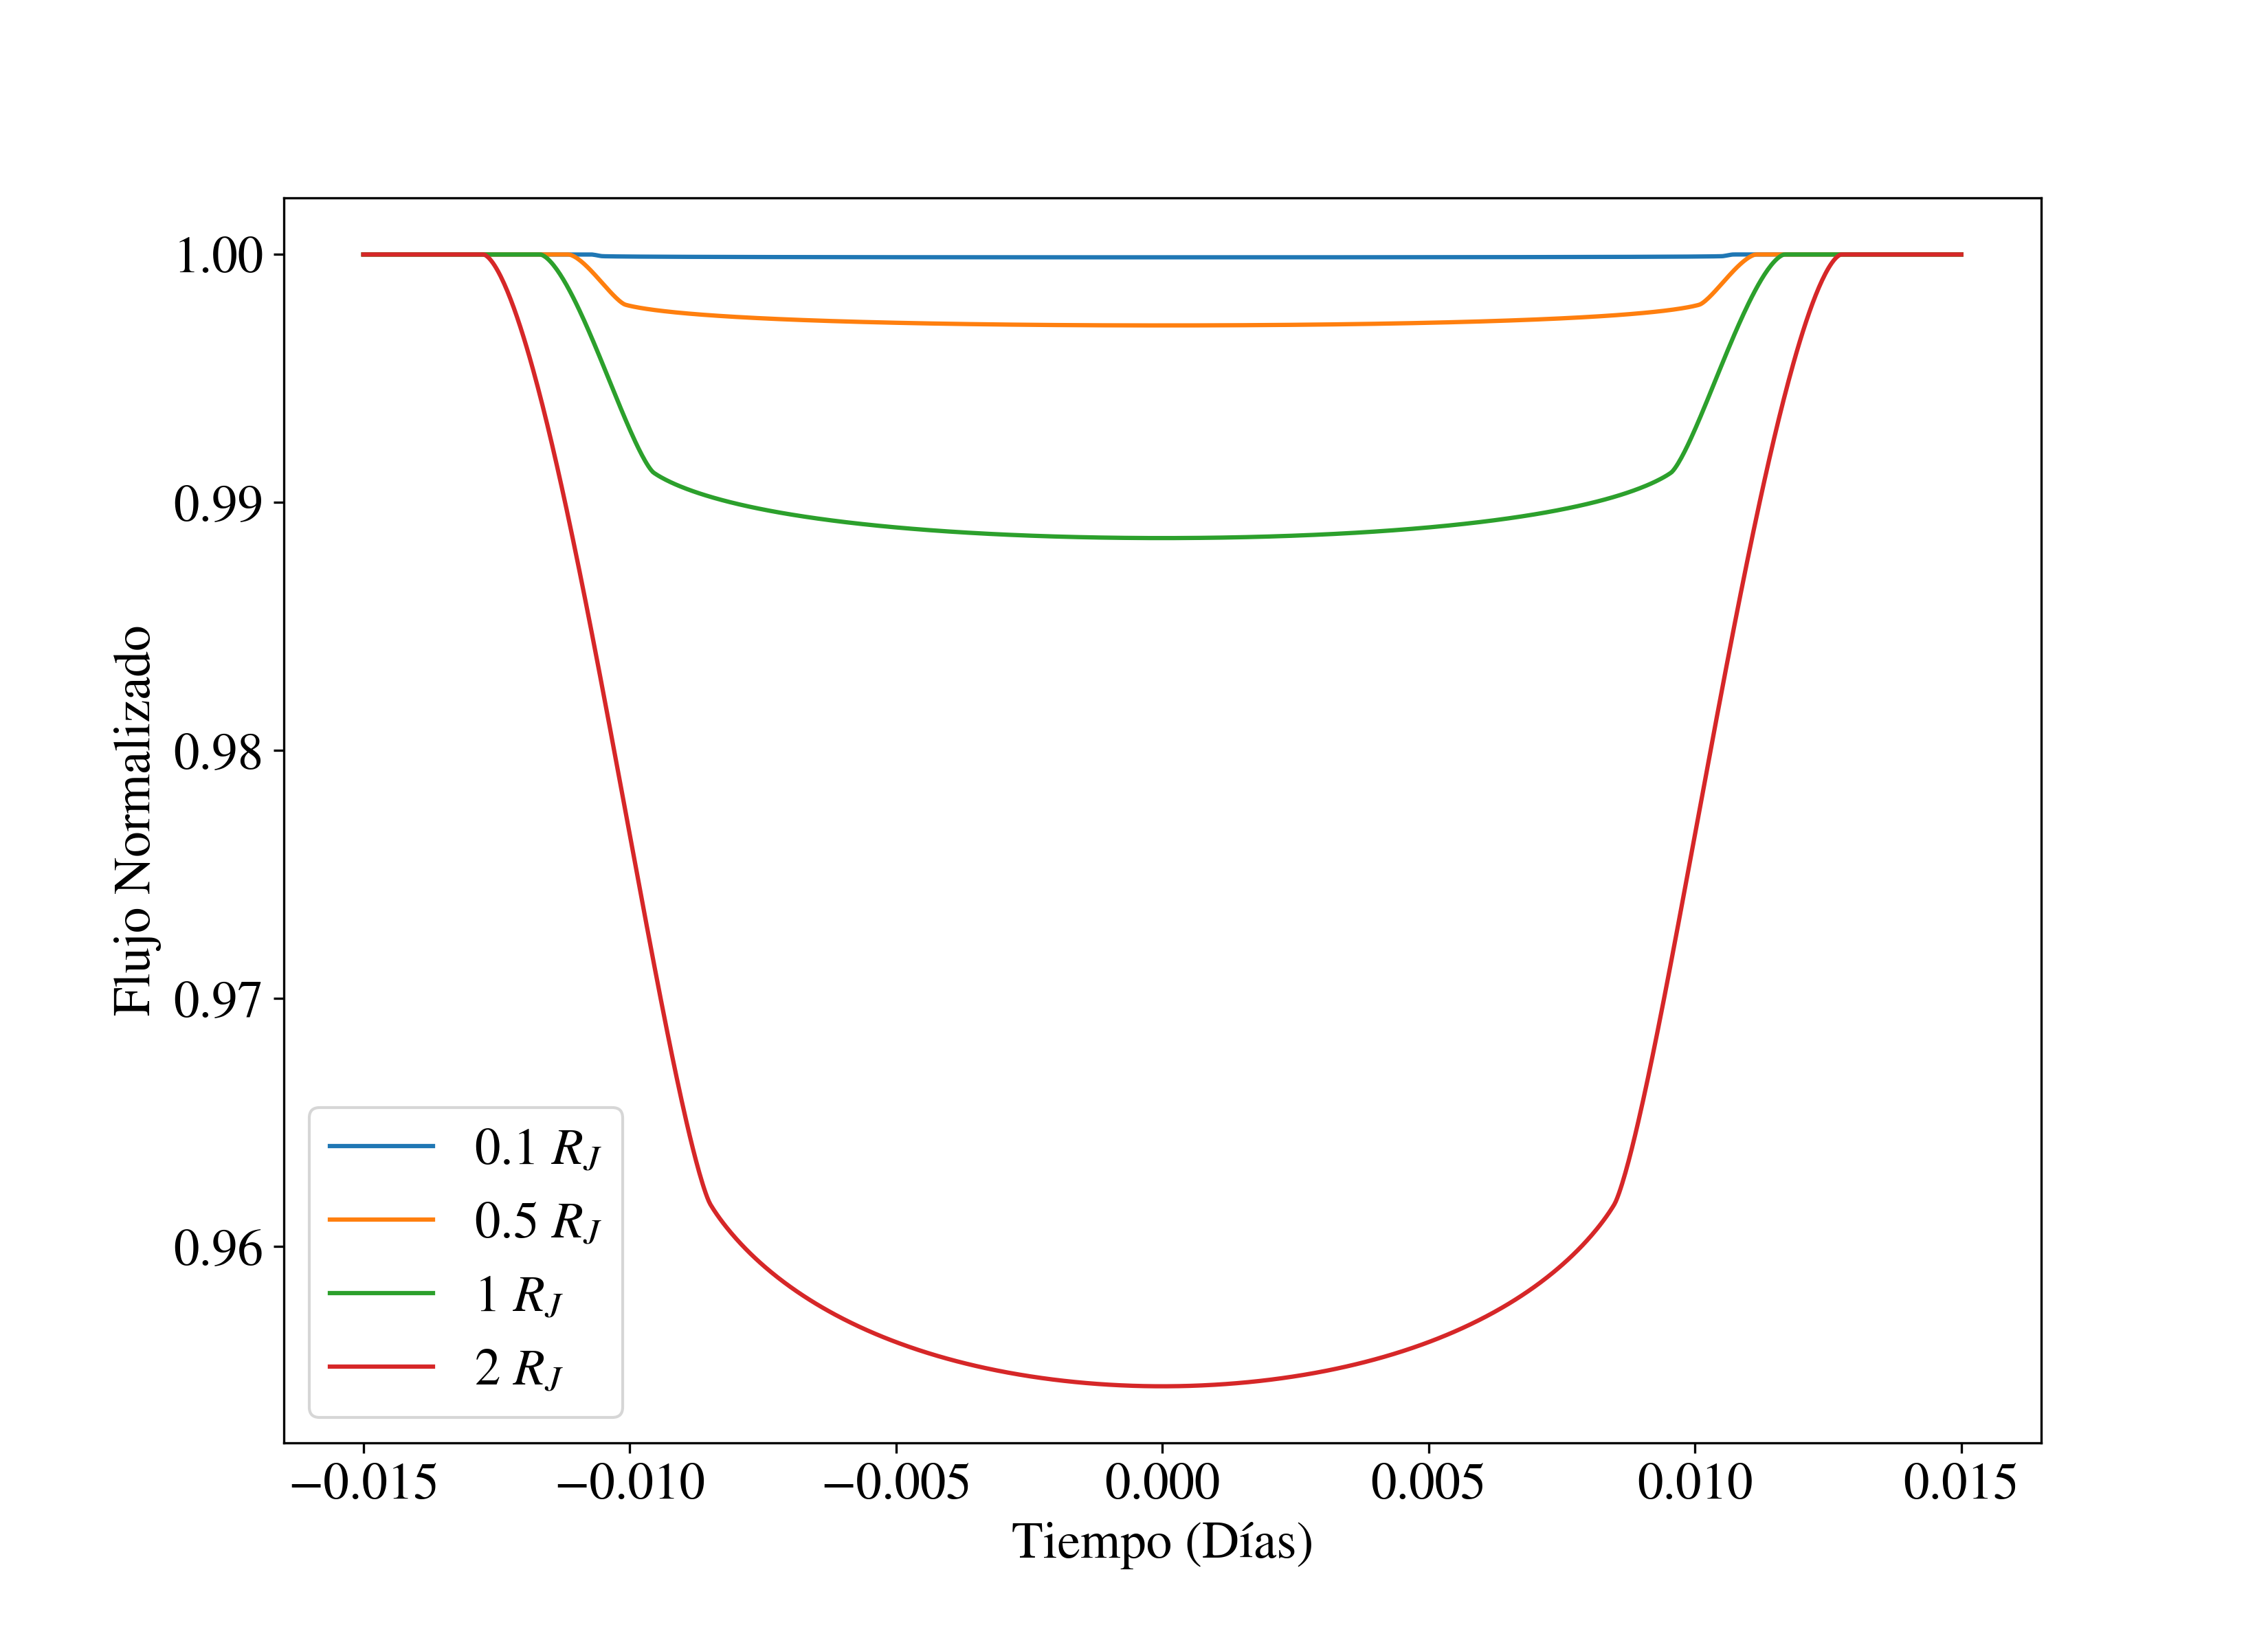
\includegraphics[max size={\textwidth}{0.65\textheight}]{./figures/transitosRadios.png}
   \caption{Fig. 3.9. Curvas de luz de tránsitos de exoplanetas con $P=1$ día, $i=90\circ$, $a=15R_{*}$, $\epsilon = 0$, $\bar{\omega}=90$ y un modelo de oscurecimiento lineal. Las distintas curvas representan la diferencia en el cambio del flujo $\Delta F$ para diferentes valores de $R_{p}$.}
    \label{fig:3.9_comp_radios}
\end{figure}

Utilizando BATMAN se creó una base de datos de tránsitos simulados, con un total de 625 curvas diferentes, utilizando 25 diferentes valores de las observables $\Delta F$ y $P$.

\section*{III.4 Análisis de datos observacionales}
\addcontentsline{toc}{section}{III.4 Análisis de datos observacionales}

En este capítulo se plantea la metodología seguida para procesar los datos observacionales resultado de las múltiples temporadas en el OAN-SPM. De los 8 objetos descritos en la sección III.1.2, se obtuvieron un total de 32 curvas de luz de alta cadencia (20 fps) y con una duración de aproximadamente 2 horas cada una. Esto con el propósito de igualar las condiciones que se tendrán en TAOS-II.

\subsection*{III.4.1 Fotometría con APPHi}
\addcontentsline{toc}{subsection}{III.4.1.1 Fotometría con APPHi}

APPHi del inglés \textit{Automated Photometry Pipeline for High Cadence, Large Volume Data} es un código desarrollado en C, el cual consta de dos principales programas, \textit{APPHi field} y \textit{APPHi star} los cuales funcionan de acuerdo al diagrama de flujo mostrado en la Figura 3.10.  Este pipeline fotométrico se utilizará como herramienta para procesar el gran volumen de datos que va generar el proyecto TAOS II \cite{lehner2016status}. Este código consta de 3 partes principales, preprocesamiento de las imágenes, localización de las estrellas en el campo de observación y la fotometría para generar las curvas de luz.

Primero las imágenes son preprocesadas de la manera convencional, utilizando imágenes de calibración (bias, flats y darks) \cite{romanishin2006introduction}. Después de limpiar las imágenes, APPHi localiza de manera automática los centroides correspondientes para cada estrella en el campo de observación usando el método del centro de masa \cite{chong2004introduction}. Este centroide se recalcula para cada imágen, para mejorar la curva de luz. Este proceso iterativo disminuye los efectos telúricos producidos por la atmósfera y el movimiento mecánico del instrumento, los cuales se vuelven significativos a altas cadencias. 

\begin{figure}[H]
  \centering
    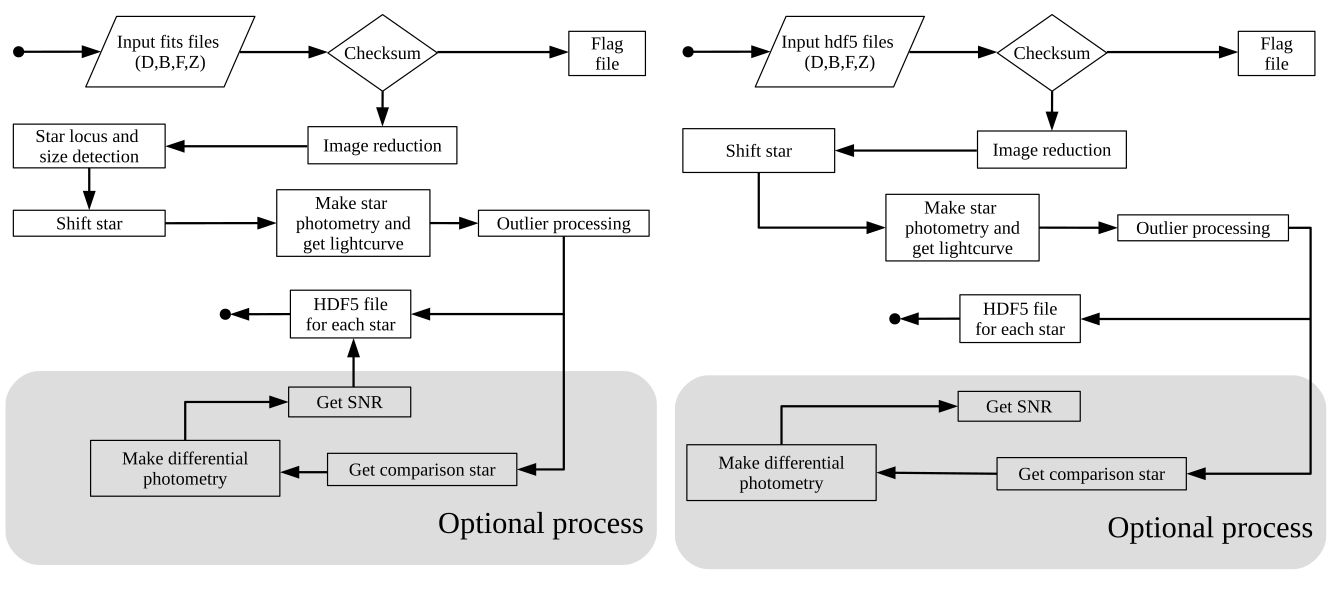
\includegraphics[max size={\textwidth}{0.7\textheight}]{./figures/apphi_diagrama.png}
   \caption{Fig. 3.10. Diagrama de flujo para ambos programas (\textit{APPHi field} y \textit{APPHi star}), donde D, B, F y Z representan los darks, bias, flats e imágenes de estudio respectivamente. Imágen tomada de \cite{sanchez2019apphi}. }
    \label{fig:3.10_aphhi_diagrama}
\end{figure}

Este proceso resulta en cubos de imágenes centradas por estrella, a partir de los cuales se realiza la fotometría de apertura. Este proceso sigue la metodología descrita en la subsección II.3.1 y en \cite{romanishin2006introduction}. 

APPHi realiza de manera automática otros procesos posteriores a la fotometría para mejorar la SNR. Uno de ellos es la fotometría diferencial, utilizando curvas de luz de estrellas cercanas como se explicó en la subsección II.3.2. Otro método que se aplica directamente a las imágenes es la técnica \textit{Shift \& Add} \cite{kluckers1996comparison}. 

Para ejecutar APPHi desde la línea de comando se utiliza:\\

\texttt{APPhi\_field bias.txt darks.txt flats.txt night.txt}\\

\noindent donde cada uno de los archivos \texttt{.txt} contiene la lista de imágenes correspondientes en formato FITS. El resultado del procesado de las imágenes es un archivo HDF5 por cada estrella en el campo de observación. Este archivo contiene las imágenes de la estrella, las coordenadas del centroide para cada imágen, la curva de luz obtenida por fotometría de apertura y fotometría diferencial \cite{sanchez2019apphi}. Todas las curvas de luz analizadas en este trabajo de tesis fueron obtenidas utilizando APPHi, el cual se encuentra disponible en \texttt{http://taos2.astrosen.unam.mx/APPHi.html}.

\section*{III.5 Reducción de ruido en curvas de luz}
\addcontentsline{toc}{section}{III.5 Reducción de ruido en curvas de luz}

Como se mencionó con anterioridad, para la detección de un tránsito exoplanetario se necesita poder medir variaciones de flujo $\Delta F \sim 1-2\%$. Lo cual en las curvas de luz de alta cadencia es difícil debido a la cantidad de ruido. En las subsecciones siguientes, se muestran los métodos para mejorar la SNR y poder identificar la presencia de un tránsito en una curva de luz.

\subsection*{III.5.1 Reducción del ruido usando promedio móvil}
\addcontentsline{toc}{subsection}{III.5.1 Reducción del ruido usando promedio móvil}

En la sección II.2 se explicó la manera convencional en el que los proyectos enfocados a la detección de exoplanetas realizan sus observaciones. Todos ellos utilizan imágenes de mediana-larga exposición, para así aumentar la SNR. Se puede intentar simular una curva de luz de larga exposición desde una de alta cadencia, simplemente integrando la contribución de $n$ muestras de la curva de luz. 

Por ejemplo, las curvas de luz de este trabajo fueron tomadas a una cadencia de 20 fps, es decir, 0.05 segundos de exposición, durante aproximadamente 2 horas, lo cual resulta en una curva $F(t)$ de $N=144,000$ muestras. Entonces, promediando el flujo de $n=1200$ muestras de la curva de luz $F(t)$, se puede simular una muestra obtenida a partir de una imágen con 60 segundos de exposición $F_{prom}(t)$ \textcolor{red}{OJO: esto no es del todo cierto, porque en una imagen de larga exposción solo lees la imagen una vez, po lo tanto el ruido electrónico juega un papel muy importante}. Es decir, cada $n=1200$ muestras de la curva de luz original, resultan en $N_{prom}=1$ muestras en la curva promediada, es decir:

\begin{equation}
  \displaystyle F_{prom}(t)=  \dfrac{\sum\limits_{i=m}^{m+n} F(t_{i})}{n}\hspace{1cm}m=0,n,2n,...,N-n;
\end{equation}

Esto resulta en una curva con longitud $N_{prom}=N/n$. Esta misma metodología aplicado a las imágenes, es el método \textit{Shift \& Add} \cite{kluckers1996comparison}.

Para evitar perder resolución temporal, se utiliza la técnica promedio móvil \cite{borucki2009kepler}. Esta técnica consiste en igualmente promediar la contribución de $n$ muestras, pero desplazando el promediado 1 muestra, en vez de $n$ como en el ejemplo anterior, es decir:

\begin{equation}
  \displaystyle  F_{mov}(t)=  \dfrac{\sum\limits_{i=m}^{m+n} F(t_{i})}{n}\hspace{1cm}m=0,1,2,...,N-n;
\end{equation}

Lo cual resulta en una curva de luz $F_{mov}(t)$ de longitud  $N_{mov}=N-n$. Otra opción análoga a este método, es usar la mediana, en lugar del promedio, esta tiene un comportamiento mas suave cuando se tienen valores atípicos. Un ejemplo del efecto de estos método en la curva de de luz de WASP-74 (Figura 3.4) se muestra en la Figura 3.11.

\begin{figure}[H]
  \centering
    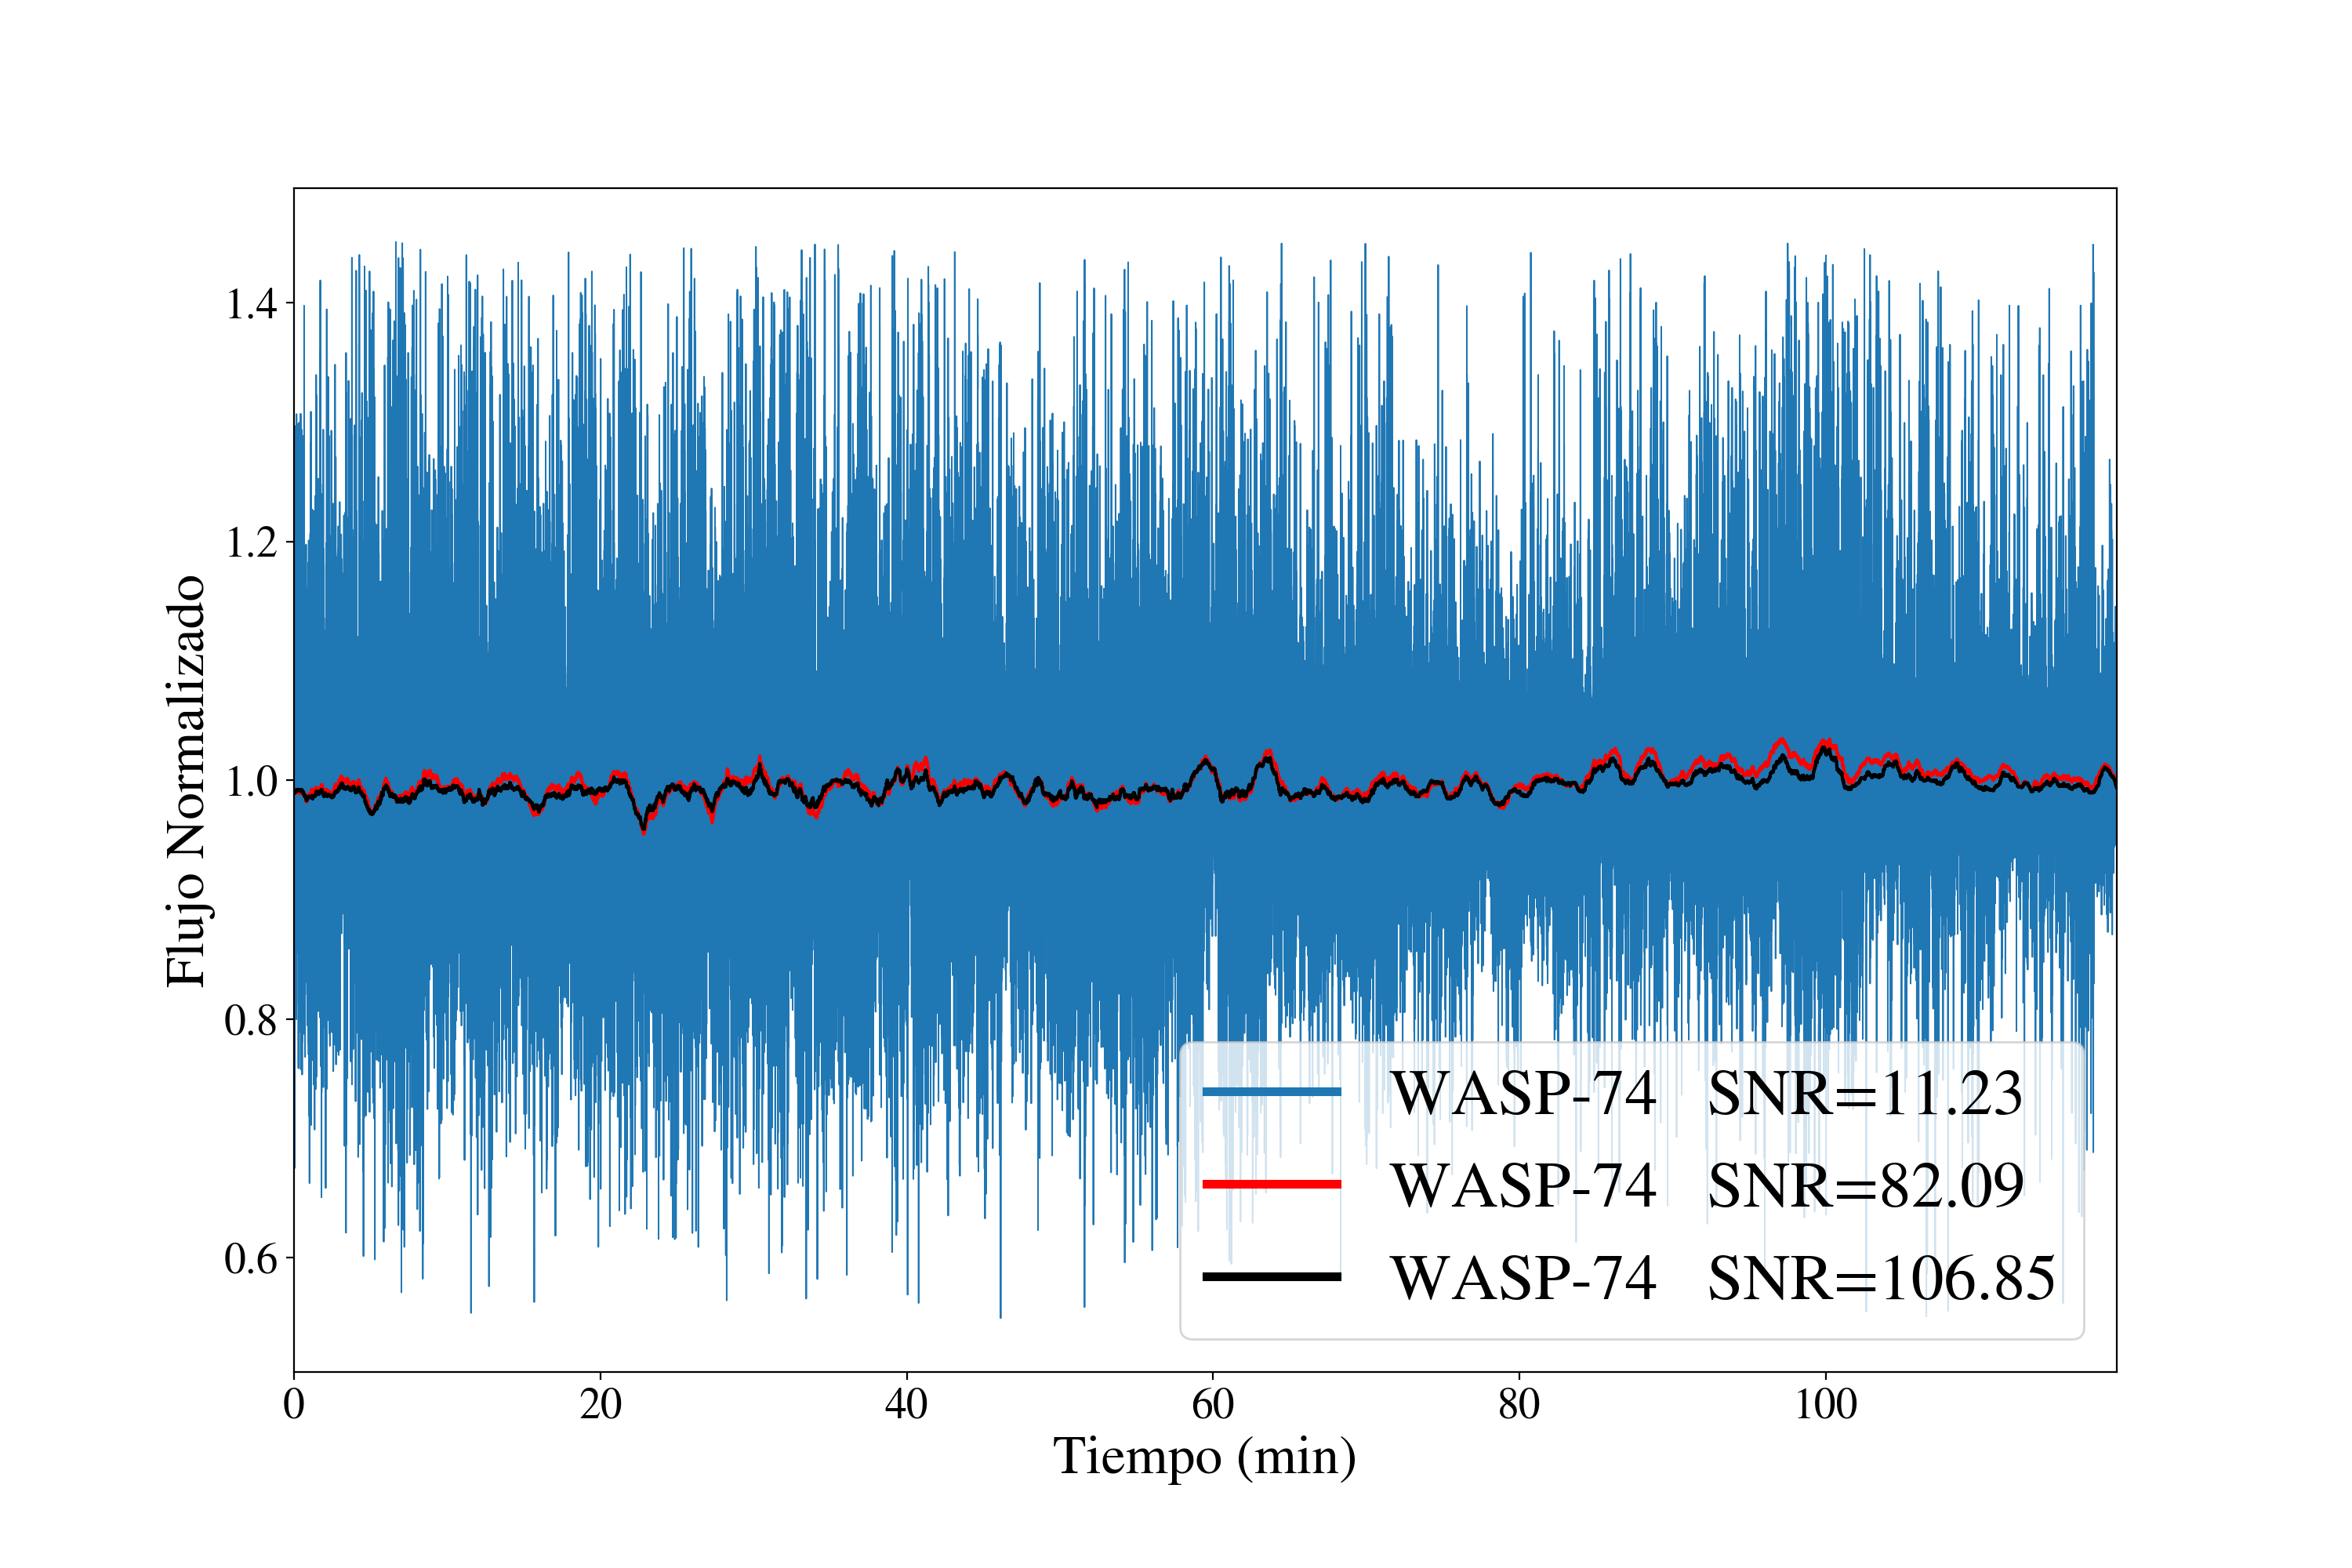
\includegraphics[max size={\textwidth}{0.7\textheight}]{./figures/wasp_prom_mov.png}
   \caption{Fig. 3.11. Curva de luz de WASP-74 tomada el día 28 de mayo del 2017. En azul se muestra la curva de luz original obtenida mediante fotometría de apertura. En naranja la curva resultado del promedio móvil, y el verde la curva resultado de tomar la mediana en lugar del promedio. En el recuadro se muestra la SNR calculada para cada curva de utilizando (2.11).  }
    \label{fig:3.11_aphhi_diagrama}
\end{figure}


\subsection*{III.5.2 Identificación de firma de tránsito usando filtro de Fourier}
\addcontentsline{toc}{subsection}{III.5.2 Identificación de firma de tránsito usando filtro de Fourier}

Un tránsito inmerso en una curva de luz de alta cadencia, puede interpretarse como una variación de baja frecuencia en el brillo de la estrella. Partiendo de esta suposición, la firma del tránsito, debe poder distinguirse en el espectro de frecuencias, particularmente en la zona de bajas frecuencias $(\sim 1x10^{-4} Hz)$.

En una curva de luz de alta cadencia, se pueden observar a simple vista variaciones de alta frecuencia, las cuales ocultan el tránsito. Estas contribuciones de alta frecuencia pueden ser atenuadas utilizando un filtro de Fourier, específicamente un filtro pasa-bajas \cite{thompson1983low}. La Figura 3.12 muestra un ejemplo del filtro pasa-bajas utilizado.

\begin{figure}[h!]
\centering
  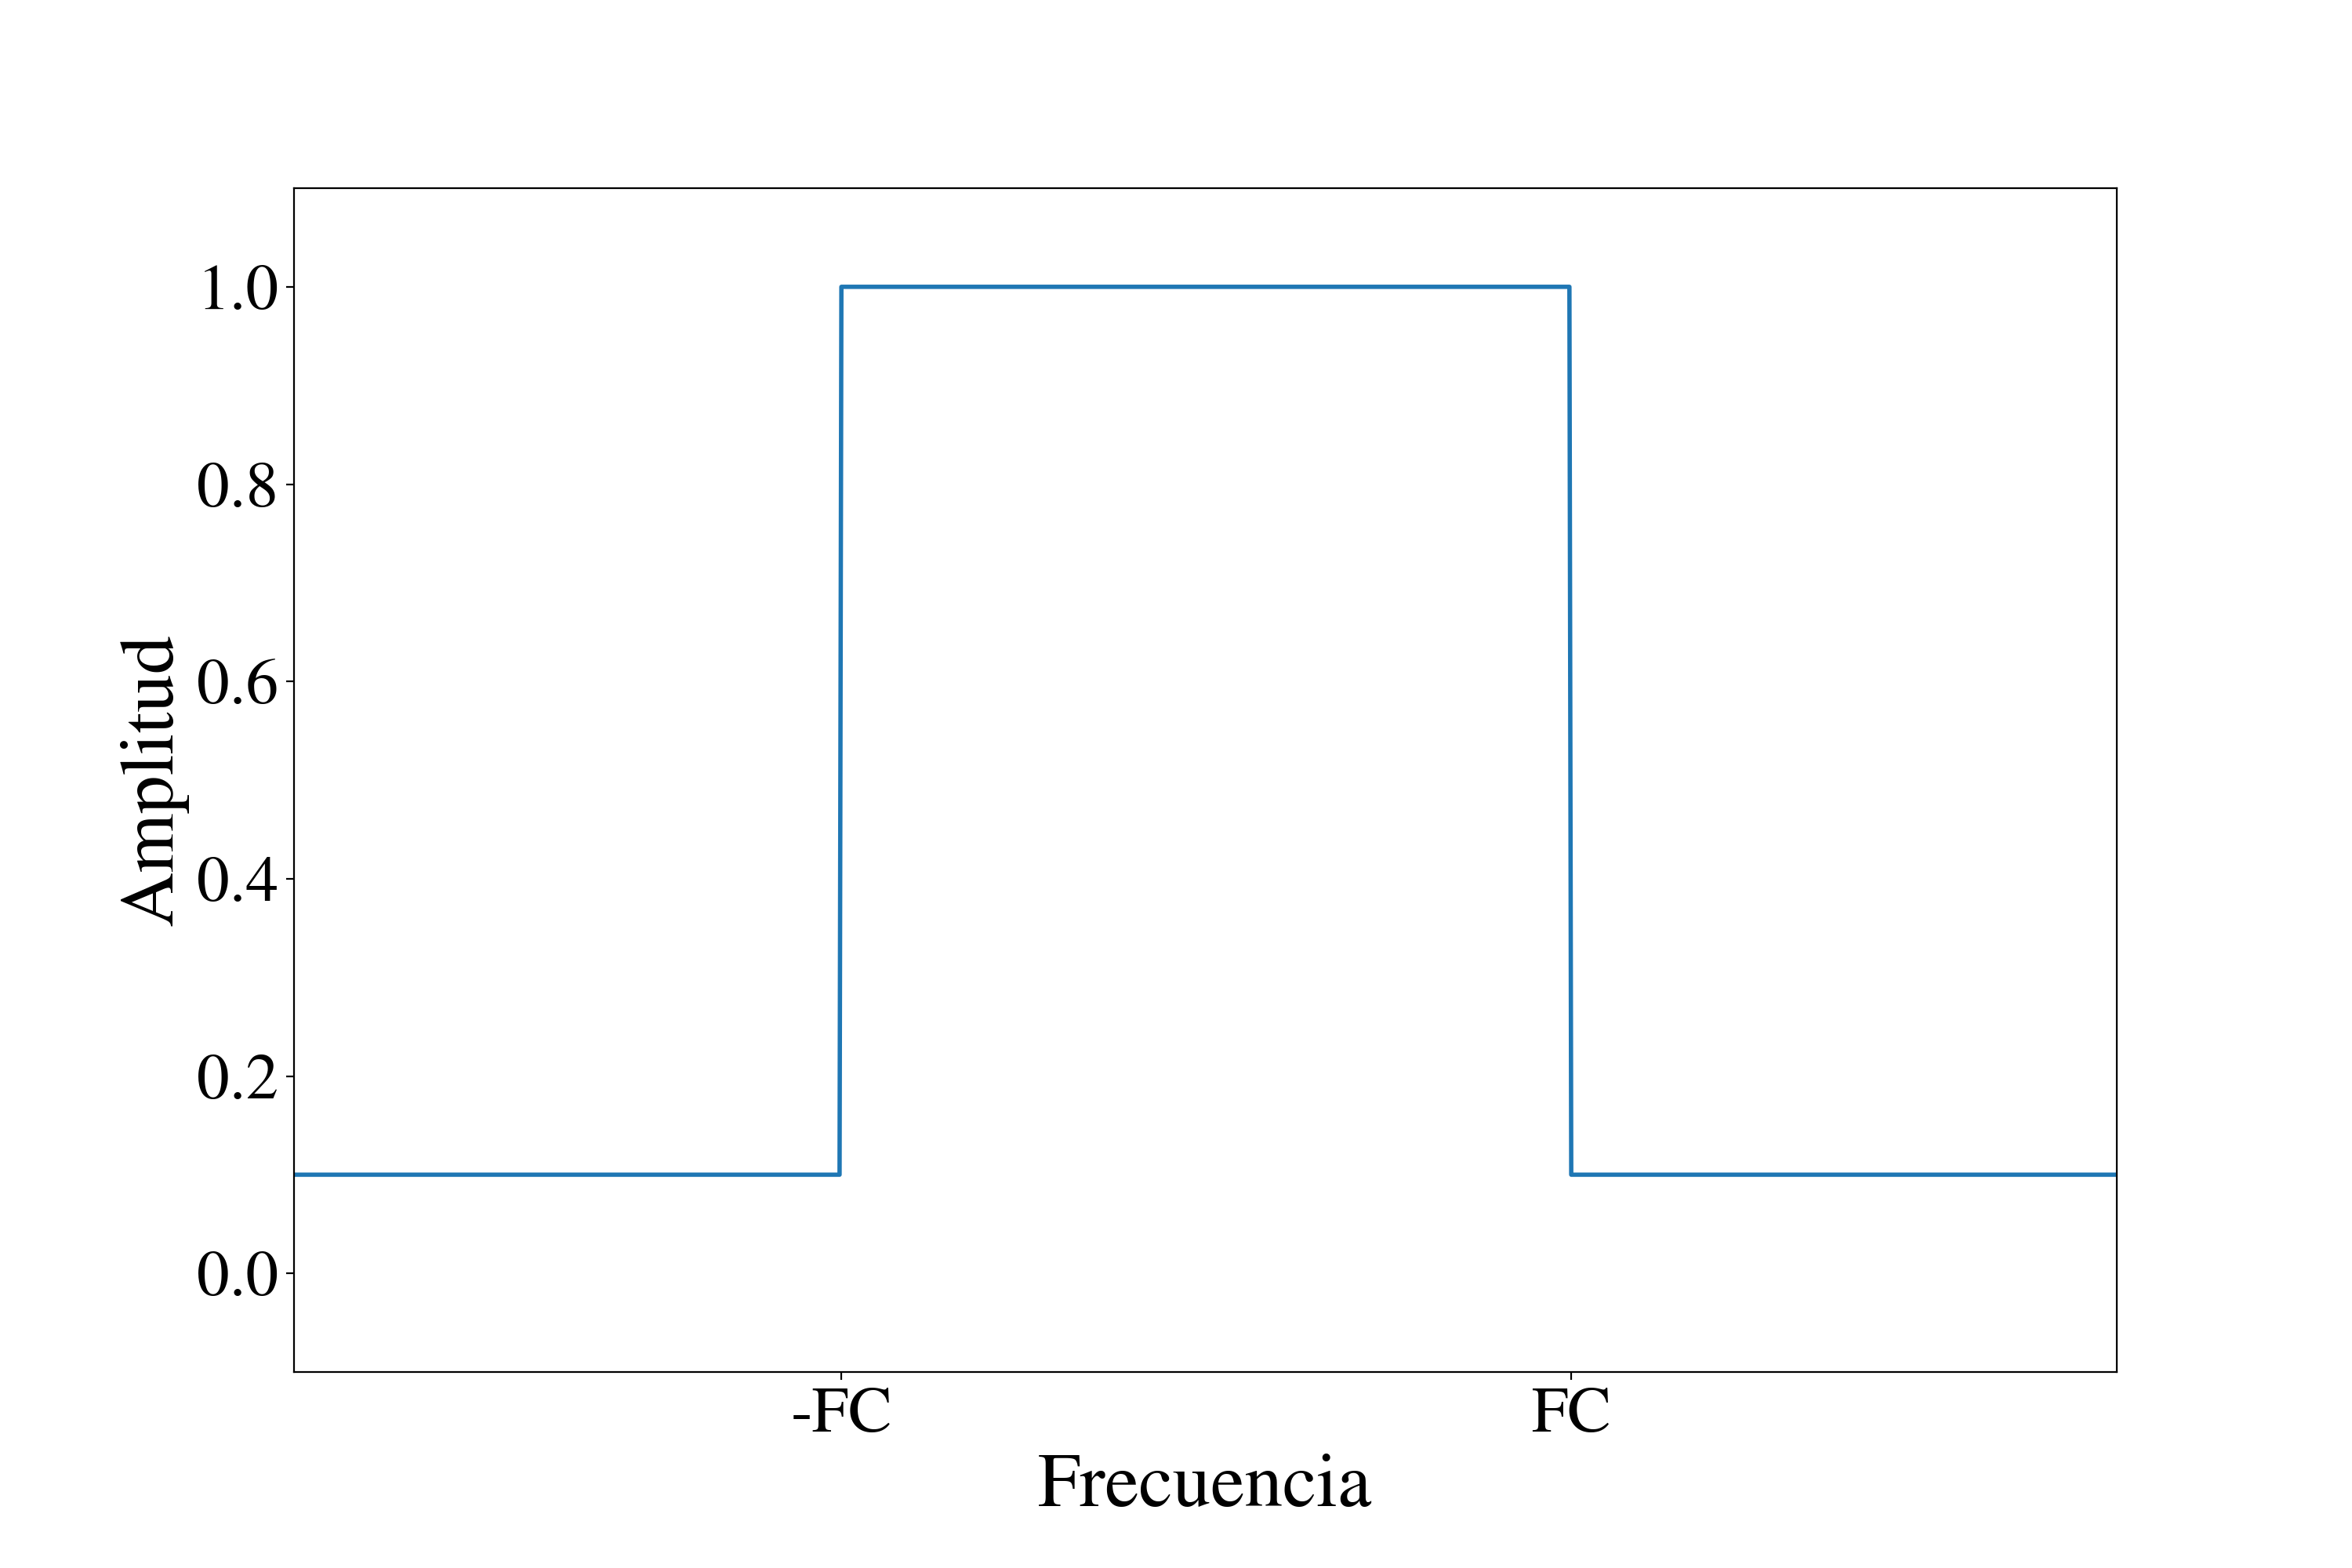
\includegraphics[max size={\textwidth}{0.7\textheight}]{./figures/filtro_pasabajas.png}
 \caption{Fig. 3.12. Filtro pasa-bajas $\mathcal{H(f)}$ utilizado para remover altas frecuencias. $FC$ representa la frecuencia de corte la cual puede variar dependiendo la curva de luz.}
  \label{fig:3.12}
\end{figure}

Para aplicar el filtro $\mathcal{H}(f)$ a $F(t)$, primero se calcula su FFT $\mathcal{F}(f)$.
Después multiplicamos el filtro, por el espectro de frecuencias para obtener el espectro filtrado $\mathcal{F}_{fil}(f)$:

\begin{equation*}
  \mathcal{F}_{fil}(f)=\mathcal{H}(f) \times \mathcal{F}(f)
\end{equation*}

finalmente regresamos al dominio del tiempo con la FFT inversa. Este proceso es análogo a utilizar una función $Sinc(t)$ como función ventana y usar la convolución en \textcolor{red}{en el dominio del tiempo} la FFT, este proceso es conocido como \textit{Windowed Fast Fourier Transform} (WFFT) \citep{owen2007practical}. Sin embargo, el proceso descrito anteriormente es computacionalmente más eficiente y obtenemos los mismos resultados, un ejemplo de la aplicación de este filtrado se muestra en al Figura 3.13.

\begin{figure}[h!]
  \centering
    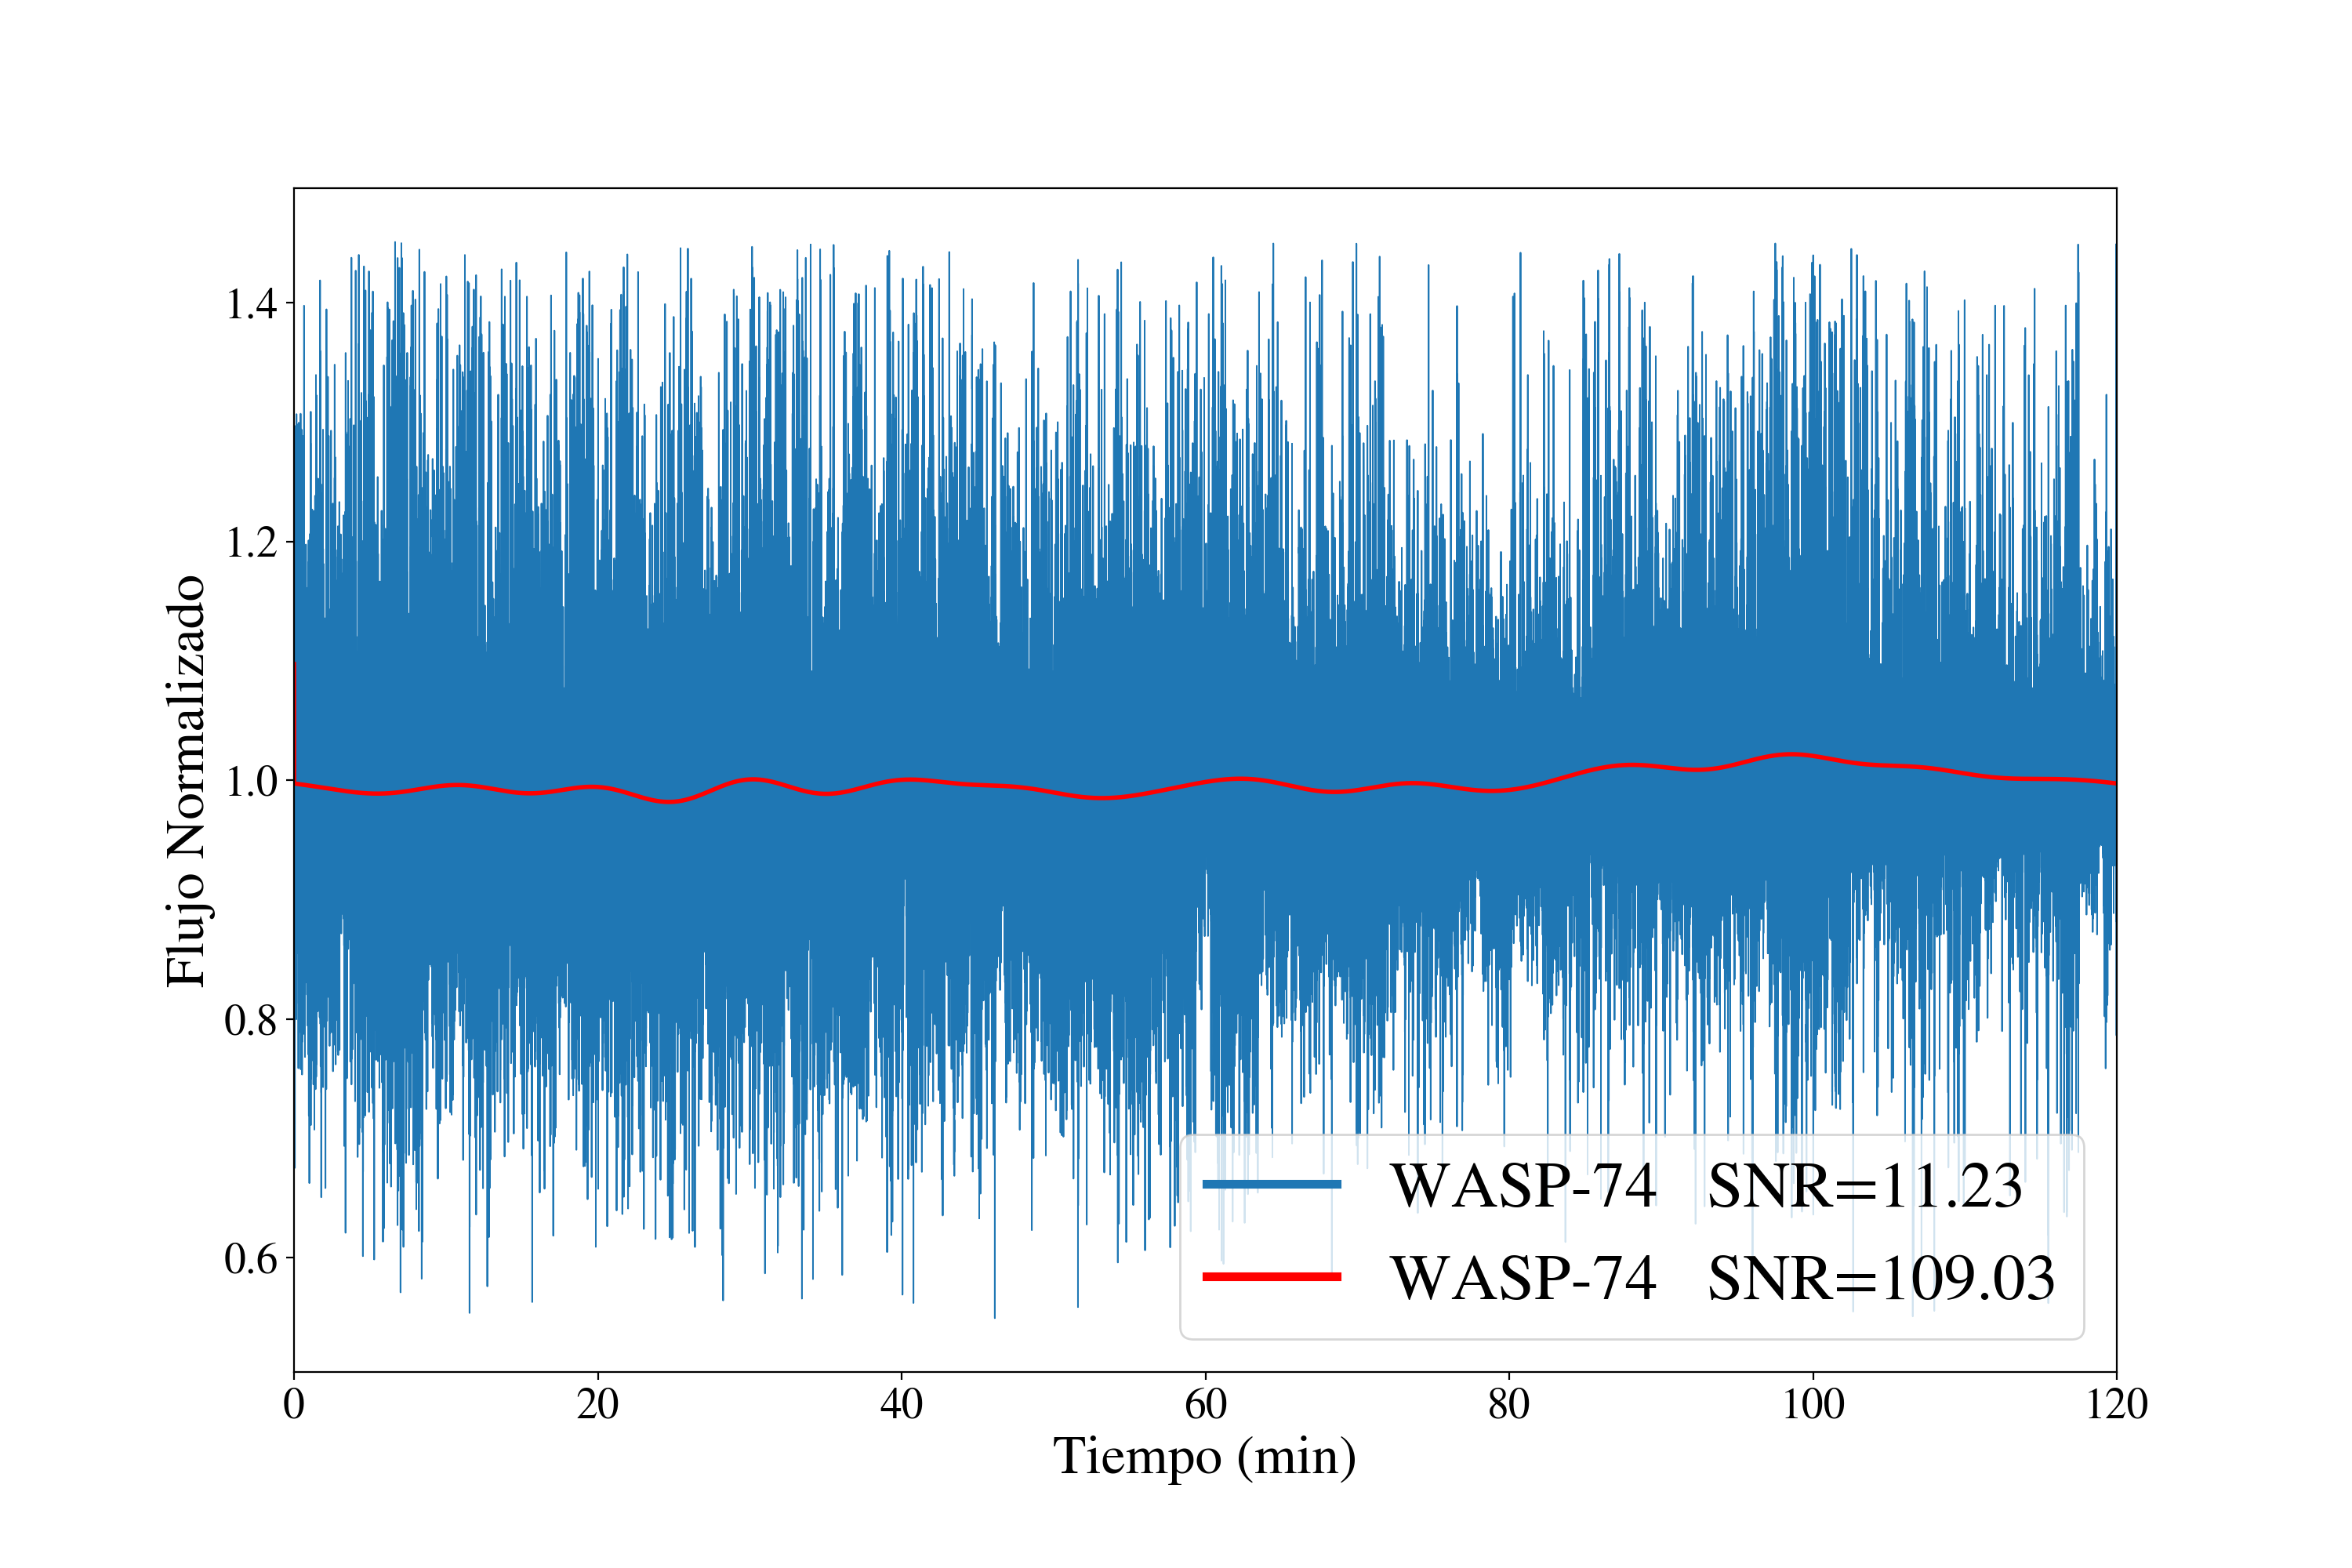
\includegraphics[max size={\textwidth}{0.7\textheight}]{./figures/wasp_four_fil.png}
   \caption{Fig. 3.13. Curva de luz de WASP-74 tomada el día 28 de mayo del 2017. En azul se muestra la curva de luz original obtenida mediante fotometría de apertura. En naranja la curva resultado del filtrado de Fourier, utilizando una frecuencia de corte $FC=2x10^{-3}$.}
    \label{fig:3.13}
\end{figure}

Este filtrado es llamado ideal por su simplicidad, sin embargo, no hay necesidad de utilizar otro tipo de funciones para $\mathcal{H}(f)$, ya que las altas frecuencias no aportan información de la firma del tránsito exoplanetario \cite{mahu2017estimation}.

\subsubsection*{III.5.3 Identificación de firma de tránsito usando PCA}
\addcontentsline{toc}{subsubsection}{III.5.3 Identificación de firma de tránsito usando PCA}

Existen metodologías para reducir el ruido en series de tiempo utilizando PCA y SVD \textcolor{red}{exoicar los acrónimos}  \cite{shin1999iterative}, \cite{bailey2012principal}. Sin embargo, el análisis de componentes principales puede emplearse de manera más conveniente, si se conocen las características de la señal que buscamos inmersa en el ruido, en este caso, tránsitos de exoplanetas.

Primero se necesita construir una matriz $X$ con muestras $\{x_{i}|i=1,...,N\}$. Cada una de estas muestras $x_{i}$, es una curva de luz de un tránsito simulado con BATMAN, con distintos periodos $(P)$ y radios de planeta $(R_{p})$:

\begin{equation}
  X = 
  \begin{pmatrix}
  x_{1} \\
  x_{2}\\
  \vdots  \\
  x_{N}
  \end{pmatrix}=
  \begin{pmatrix}
    v^{1}_{1} & v^{1}_{2} & \cdots & v^{1}_{n} \\
    v^{2}_{1} & v^{2}_{2} & \cdots & v^{2}_{n} \\
    \vdots  & \vdots  & \ddots & \vdots  \\
    v^{N}_{1} & v^{N}_{2} & \cdots & v^{N}_{n} 
  \end{pmatrix}
\end{equation}

donde $n$ es el número de puntos en la curva simulada $\{v^{N}_{i}|i=1,...,n\}$. Por cual entonces, $X$ tiene dimensiones $N\times n$, y su SVD está dada por:

\begin{equation}
  \displaystyle X=U\Sigma V^{T};
\end{equation}

Para calcular la matriz de eigenvalores $V^{T}$, se utilizó la función \texttt{TruncatedSVD} de la paquetería \textit{Scikit Learn} en \textit{Python}. Como su nombre lo indica, esta SVD esta truncada a las primeras $k$ componentes más significativas, donde $k$  es definido por el usuario. Esta función nos proporciona la matriz $V^{T}$ truncada, de dimensiones $k\times N$.

Después se calcula la contribución de las $k$ componentes sobre una curva de luz $F_{t}$ o un conjunto de $l$ curvas de luz:

\begin{equation}
  \displaystyle C=V^{T} \times F_{t};
\end{equation}

donde C tiene dimensiones $k\times l$, si utilizamos una sola curva de luz $l=1$. Finalmente para construir la curva de luz $F'_{t}$ reconstruida en base a las $k$ componentes principales:

\begin{equation}
  \displaystyle F'_{t}=C^{T} \times V^{T};
\end{equation}

Este proceso utiliza las componentes principales de los tránsitos simulados para recontruir la curva de luz con ruido. Esto no es análogo a una reducción de ruido. Si la curva $F_{t}$ que se va analizar no contiene las características que se están buscando (las características de $X$), el resultado es una curva $F'_{t}$ que no posee ningún patrón específico. Esto no se convierte en un problema, dado que solo estamos interesados a las curvas que sí presenten las características de un tránsito.


\section*{III.6 Criterio de validación para candidatos a tránsitos de exoplanetas}
\addcontentsline{toc}{section}{III.6 Criterio de validación para candidatos a tránsitos de exoplanetas}

Las curvas de luz que resultan de las metodologías para reducción de ruido y PCA, son analizadas de manera automática, donde se ajusta un modelo para validar si es un posible candidato a tránsito de exoplaneta o no. \textcolor{red}{hacer mas amigable este parrafo}

\subsection*{III.6.1 Modelo del trapezoide}
\addcontentsline{toc}{subsection}{III.6.1 Modelo del trapezoide}

Las curvas de luz de alta candencia son mucho mas tardadas de procesar por el número de mediciones que se realizan. Como se mencionó anteriormente, TAOS-II tendrá curvas de luz de 2 horas de longitud, lo cual se traduce en curvas con $N=144,000$ muestras. Además, por campo de observación se espera observar alrededor de 10,000 estrellas simultaneamente. Teniendo en cuenta la eficiencia del algoritmo, se utilizó el modelo más simple para un tránsito de exoplaneta, un trapezoide. Este modelo es muy utilizado en el procesamiento de señales producidas por tránsitos de exoplanetas, por ejemplo los trabajos \cite{alapini2010transiting}, \cite{hippke2019optimized}, \cite{kipping2016observational} y \cite{morton2012efficient}.


Como se explicó en la sección II.1, a partir de curvas de luz de tránsitos solo podemos conocer el periodo orbital $P$ y la profundidad del tránsito $\Delta F$, la cual está en función del radio del planeta $R_{p}$ y el radio de la estrella $R_{*}$. Por lo que el modelo del trapezoide es suficiente para validar un posible candidato a tránsito.

\subsection*{III.6.2 Coeficiente de correlación de Pearson}
\addcontentsline{toc}{subsection}{III.6.2 Coeficiente de correlación de Pearson}

Después de ajustar el modelo del trapezoide a las curvas de luz, se utilizó el coeficiente de correlación de Pearson, para evaluar la calidad del ajuste. 

\begin{equation}
\displaystyle C=\frac{\sigma_{12}}{\sigma_{1}\sigma_{2}};
\end{equation}
  
donde $\sigma_{12}$ es la covarianza entre la curva de luz y el modelo ajustado, definida como:
  
\begin{equation}
\displaystyle \sigma_{xy}= \sum\limits_{i}^{n} \frac{1}{n}(x_{i}-\bar{x})(y_{i}-\bar{y});
\end{equation}
  
donde $\sigma_{1}$ y $\sigma_{2}$ son la desviación estándar de la curva de luz y el modelo respectivamente. A partir de simulaciones, se calculó el limite inferior para el coeficiente de correlación, para evaluar si la estrella y su curva de luz se cataloga como objeto de interés, para elaborar un análisis más detallado (véase IIII.2 \textcolor{red}{que numero de seccion es ese??}).